
\FloatBarrier

\section{Система Лоренца} % {{{1_LOR_
\label{atu:sect:lor}

\LinkRef{
  lor: ASAU-22, 23, 24, 25, 26.
  % ~/doc/tex/asau/asau22/atu/atu.tex
  % ~/doc/tex/asau/asau23/atu/atu.tex
  % ~/doc/tex/asau/asau24/atu/atu.tex
  APIR-2012. CSIT-2015. ISDMCI-2014, ISDMCI-2015.
  ITMM-2012, ITMM-2014, ITMM-2015, DSMP-2016
}

\subsection{Визначення системи та аналіз її динаміки}%%{{{2_LOR_task

У якості першої ідентифікованої хаотичної системи розглянемо класичну систему
Лоренца, динаміка якої описується системою
рівнянь:~\cite{moon_chaotic_vibr,anisch_nonlin_eff,chulichkcov_mm_ml_dyn,berje_order_in_chaos}:
%
\begin{equation}
\begin{cases}
  \dot{x} = \sigma (y-x ) , \\
  \dot{y} = x (r-z) - y , \\
  \dot{z} = x y - b z .
\end{cases}
\label{atu:eq:lor}
\end{equation}

Найціннішим з точки зору ідентифікації є параметр $r$, що визначає як
енергетичний стан системи, так і вид динаміки системи. Це підтверджують і
фізичні обґрунтування. Для визначеності задамо інші параметри наступним
класичним чином: $b = 8/3$, $\sigma = 10$, якщо не буде явно
зазначено протилежне.


При малих значеннях параметра $r$ система демонструє затухаючі коливання
(рис.~\ref{atu:f:lor_attractor_fading}).

\begin{figure}[ht!]
\begin{center}
  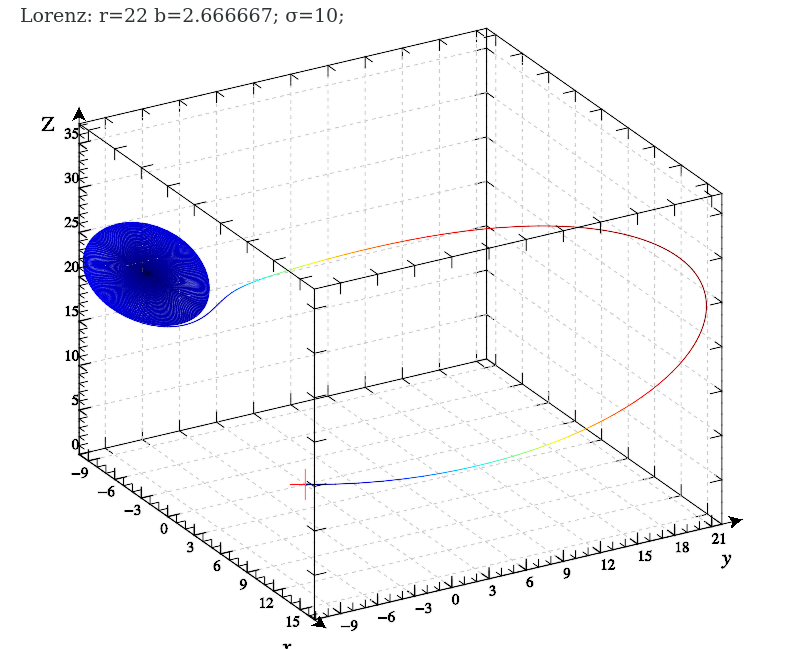
\includegraphics[width=0.49\textwidth]{p/cha/lor/lor0-p_xyz_r=022.png}
  \hfill
  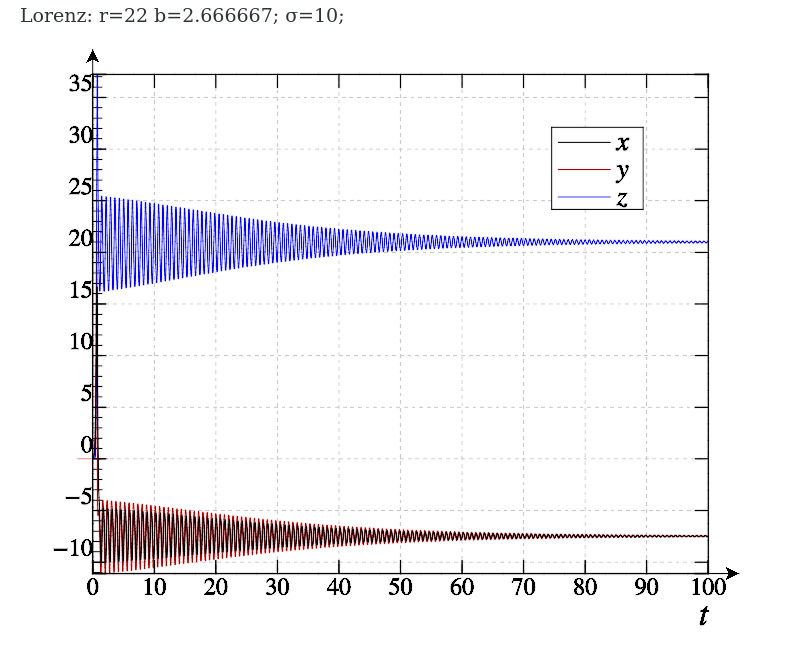
\includegraphics[width=0.49\textwidth]{p/cha/lor/lor0-p_t_r=022.png}
\end{center}
\caption{Аттрактор і поведінку змінних стану системи Лоренца (\ref{atu:eq:lor}) в режимі затухаючих коливань ( $ r = 22 $)}
\label{atu:f:lor_attractor_fading}
\end{figure}

Далі, в широкому діапазоні значення параметра $r$ система проявляє хаотичну
динаміку. Крім цього, спектр даної системи в хаотичному режимі досить широкий
(рис.~\ref{atu:f:lor_attractor_phase_chaos28}) і не має домінуючих
частот, що не характерно для багатьох систем динамічного хаосу.

\begin{figure}[ht!]
\begin{center}
  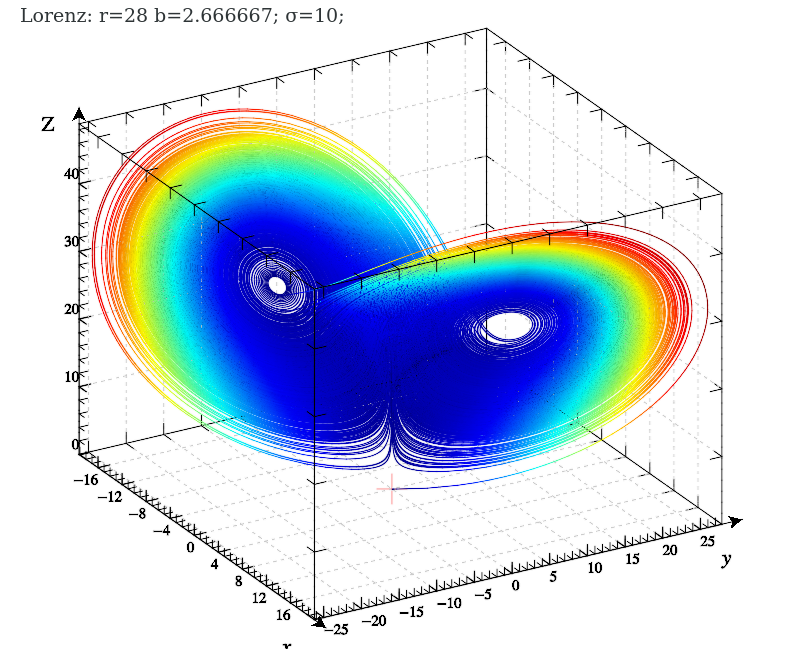
\includegraphics[width=0.49\textwidth]{p/cha/lor/lor0-p_xyz_r=028.png}
  \hfill
  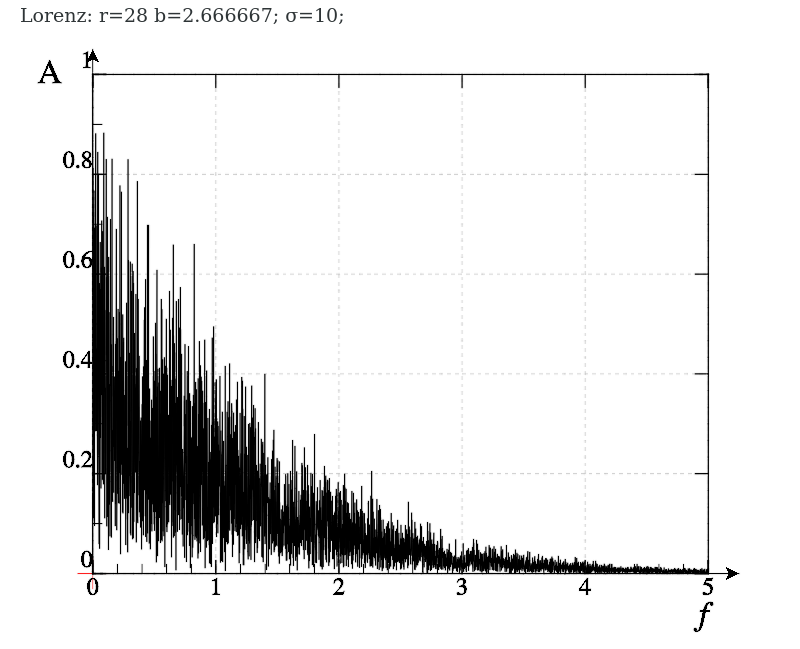
\includegraphics[width=0.49\textwidth]{p/cha/lor/lor0_fft-p_f_r=028.png}
\end{center}
\caption{Аттрактор і спектр системи Лоренца (\ref{atu:eq:lor}) в хаотичному режимі ($ r = 28 $)}
\label{atu:f:lor_attractor_phase_chaos28}
\end{figure}

При подальшому зростанні параметра $r$ динаміка системи стає
складно-періодичною, з явно вираженим лінійчатим спектром
(рис.~\ref{atu:f:lor_attractor_phase_200}).

\begin{figure}[ht!]
\begin{center}
  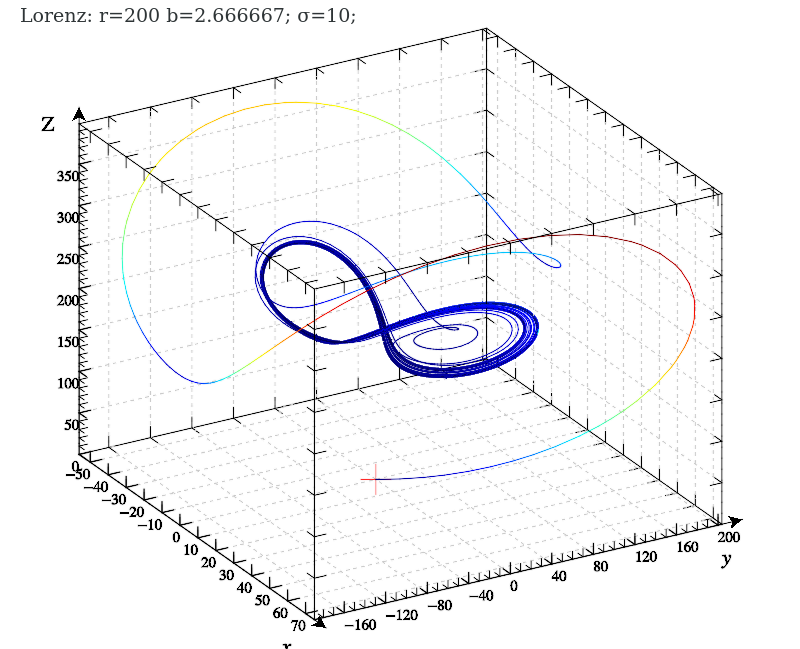
\includegraphics[width=0.49\textwidth]{p/cha/lor/lor0-p_xyz_r=200.png}
  \hfill
  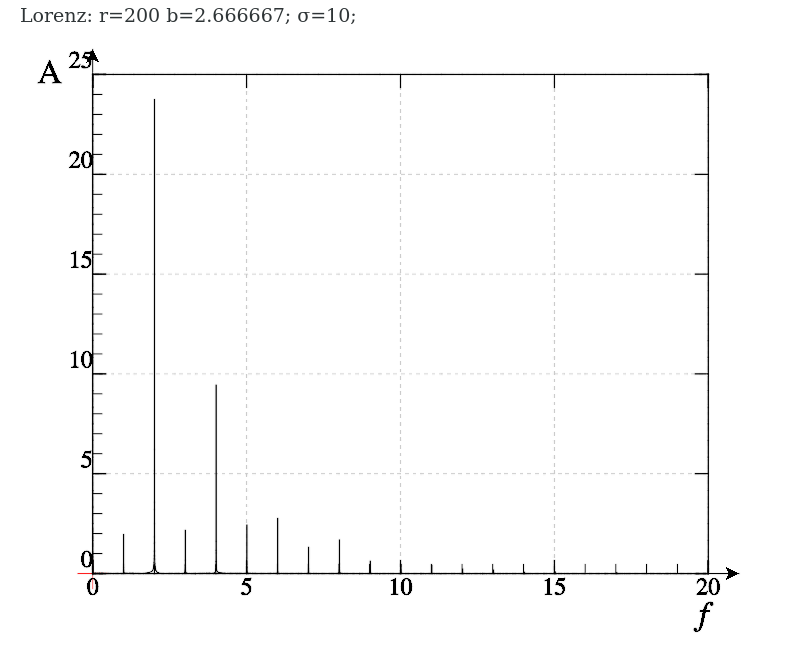
\includegraphics[width=0.49\textwidth]{p/cha/lor/lor0_fft-p_f_r=200.png}
\end{center}
\caption{Аттрактор і спектр системи Лоренца (\ref{atu:eq:lor}) в складно-періодичному режимі ($r = 200 $)}
\label{atu:f:lor_attractor_phase_200}
\end{figure}



Динамічна система Лоренца є однією з найбільш досліджених
хаотичних систем~\cite{neimark_stoch_chaos_vibro}. При цьому, існує множина
фізичних систем, для опису яких може бути застосована модель
Лоренца. Це дає певні підстави припускати, що синтез критерію
ідентифікації, заснованого на фізичних принципах, для даної
системи буде успішним.


Для синтезу крітерію ідентіфікації параметра
$ r $ системи (\ref{atu:eq:lor}), розглянемо набір фізичних систем, для
моделювання якіх застосовується система Лоренца.

Історично першою такою системою є задача про теплову
конвекцію рідини в плоскому шарі.
%
Початкова система рівнянь гідродинаміки має вигляд:
%
%
\begin{equation}
\begin{cases}
  \pd{\vec{v}}{t} + ( \vec{v} \nabla ) \vec{v} = - \frac{\nabla p}{\rho} + \nu \Delta \vec{v} + \vec{g}, \\
  \pd{\rho}{t} + \nabla ( \rho \vec{v} ) = 0 , \\
  \pd{T}{t} +\nabla ( T \vec{v} ) = \chi \Delta T , \\
  \rho = \rho_0 \left( 1 - \gamma (T - T_0) \right) .
\end{cases}
\label{atu:eq:lor_gidro}
\end{equation}
%
де
$ \Vec{v} $ --- поле швидкостей,
$ T $ --- поле температури,
$ T_0 $ і $ T_0 + \Delta T $ --- температури на верхній і нижній межі відповідно,
$ \rho $ і $ p $ --- поля щільності і тиску,
$ g $ --- прискорення вільного падіння,
$ \nu $,
$ \chi $,
$ \gamma $ --- коефіцієнти кінематичної в'язкості,
температуропроводности і теплового розширення відповідно.

Змінні і параметри системи (\ref{atu:eq:lor_gidro}) при приведенні к виду~(\ref{atu:eq:lor})
визначаються наступним чином:
$x$ задає швидкість обертання валів течії,
$y$, $z$ --- відповідають розподілу температури по горизонталі і вертикалі.
$\sigma$ --- число Прандтля (відношення коефіцієнтів кінематичної в'язкості і температуропроводності).
Параметр $b$ визначає відношення розмірів осередку,
$r$ --- (ідентифікований параметр) --- приведене число Релея, що визначає енергетичні параметри
конвективної течії.

З трьох змінних стану найпростішому спостереженню піддається змінна $x$.
З іншого боку, оскільки параметр $r$ визначає енергетичні співвідношення в
системі, то і критерій якості повинен являти собою квадратичну форму від $x$,
причому усереднену на інтервалі часу, значно більшому, ніж характерний час
обороту рідинного вала.

Іншою системою, для моделювання якої застосовується система
Лоренца --- це модель одномодового лазера~\cite{andrianov_laser}. У цій
моделі змінної
$ x $ відповідає амплітуда поля в резонаторі,
$ y $ --- поляризації,
$ z $ --- інверсії заселеності квантових рівнів активного середовища. Параметри
$ \sigma $ і $ b $ визначаються відносинами коефіцієнтів релаксації, а шуканий
параметр
$r$ визначається питомою потужністю накачування.

Як і в разі гідродинамічної системи, найбільш просто
спостережуваним параметром є
$x$ --- саме він визначає вихідну інтенсивність. І знову ж таки,
за аналогією --- ідентифікований параметр
$r$ визначає енергетику системи. При переході від амплітуди
до потужності абсолютно аналогічно слід використовувати
квадратичну залежність.

Також система (\ref{atu:eq:lor}) може бути застосована для моделювання
конвекції рідини в замкнутому підігрівається петлі, динаміки
водяного колеса, осцилляторе з тертям
та інших~\cite{kuznetsov_dyn_chaos,atu_arsirii}.

% }}}2


\subsection{Аналіз і вибір критеріїв} % {{{2

Виходячи з вищевикладеного, в першу чергу слід перевірити придатність критерію
виду $q_{x^2}$~\cite{atu_apir2012}.
Проте перевіримо всі критерії даного виду, застосовні до
даної системи. На рис.~\ref{atu:f:lor_q} наведені залежності
$q_{*}(r)$, які були досліджені.

На рис.~\ref{atu:f:lor_q} наведені досліджувані залежності
$q(r)$, отримані шляхом моделювання динаміки системи (\ref{atu:eq:lor})
для різних значень параметра~$r$, при усередненні на значному часовому інтервалі
$ \tau_q = 500 $.


\begin{figure}[ht!]
  \centerline{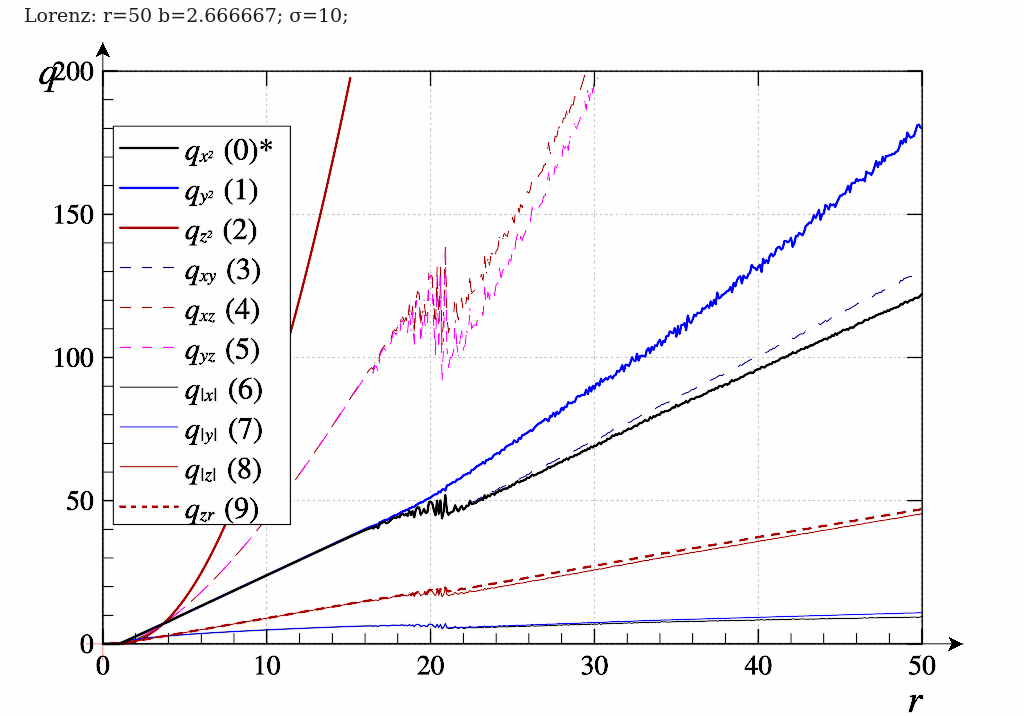
\includegraphics[width=0.7\textwidth]{p/cha/lor/lor_q-p_q_r.png} }
  \caption{Розглянуті критерії для системи Лоренца}
  \label{atu:f:lor_q}
\end{figure}

З аналізу графіків зроблено висновок, що практично всі розглянуті види
критеріїв повинні дозволяти побудувати працездатну систему ідентифікації. При
цьому, велика частина графіків, в тому числі і з самого початку запропонований
$q_{x^2}$, втрачають монотонність при переході від режиму загасаючих
коливань до хаотичного.
що може перешкодити процесу ідентифікації поблизу цієї
точки. Проте, режим згасаючих коливань не представляє
практичного інтересу, і цим недоліком можна знехтувати. Цього
недоліку позбавлений критерій
$ q_{y^2} $, проте, в даних фізичних задачах значення
$ y (t) $ спостерігати складніше. Критерій
$ q_{z^2} $ має явно виражену параболічну форму, а критерії
$ q_{zr} $ і
$ q_{|z|} $ також є потенційними кандидатами в застосовні
критерії. Критерії виду
$ q_{xy} $,
$ q_{xz} $ і
$ q_{yz} $ мало придатні через високий рівень коливань.

Спектри сигналів $x(t)$, $y(t)$ і $z(t)$ мають практично однакову
структуру. У подальших дослідженнях використовувалися критерії
$q_{x^2}$ та
$q_{y^2}$.

Наступна залежність, необхідна для синтезу системи
ідентифікації ---
$ \sigma_q (\tau_q) $ або ж
$ \sigma_q (a_q) $ --- співвідношення між часом оцінювання
$ \tau_q $ і середньоквадратичної похибкою вимірювання критерію. Для
моделювання безпосередніх похибок вимірювання величин
$ x (t) $ і
$ y (t) $ використовувався шум з нормальним розподілом і
параметрами
$ \sigma_w = 0.5 $ і
$ \tau_w = 0.05 $~\cite{atu_asau26}.

Для оцінювання необхідної залежності, для кожного значення
$ \tau_q $ з заданого діапазону проводилося
$ N = 200 $ процесів моделювання динаміки системи, і в випадковий
момент (досить далеко віддалений від точки
$ t = 0 $ для виключення крайових ефектів) проводилося вимірювання
і запам'ятовування значення обраного критерію. При цьому, для усереднення
величини
$ q $ використовувалося 2 методу: експоненціальне згладжування,
виду (\ref{atu:eq:qlin}), і ковзне середнє~(\ref{atu:eq:moving_avarage}). Отримані
залежності, позначені відповідно
$ \sigma_{ql} $ і
$ \sigma_{qa} $, представлені на рис.~\ref{atu:f:lor_qy2_tau} і~\ref{atu:f:lor_qx2_tau}.


\begin{figure}[ht!]
\begin{center}
  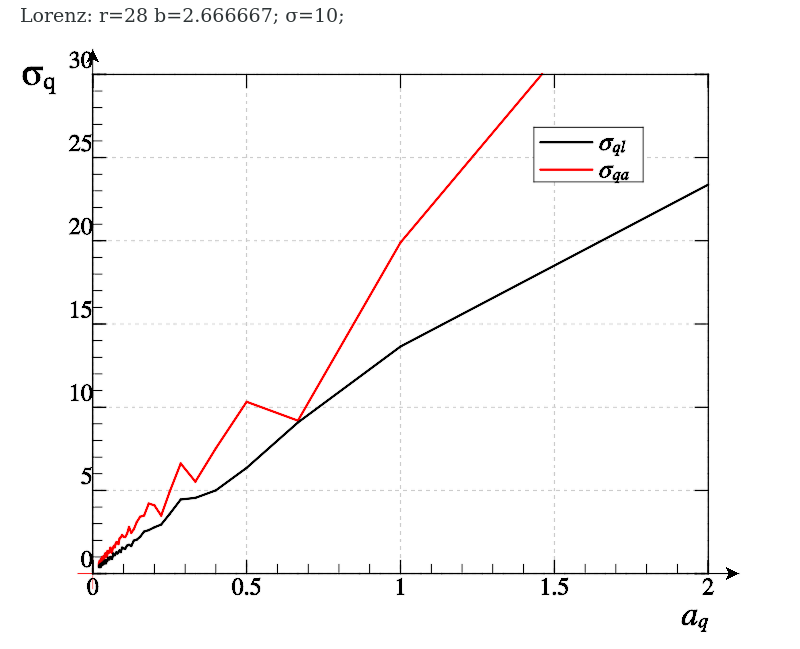
\includegraphics[width=0.49\textwidth]{p/cha/lor/lor_q_tau-p_aq_sd.png}
  \hfill
  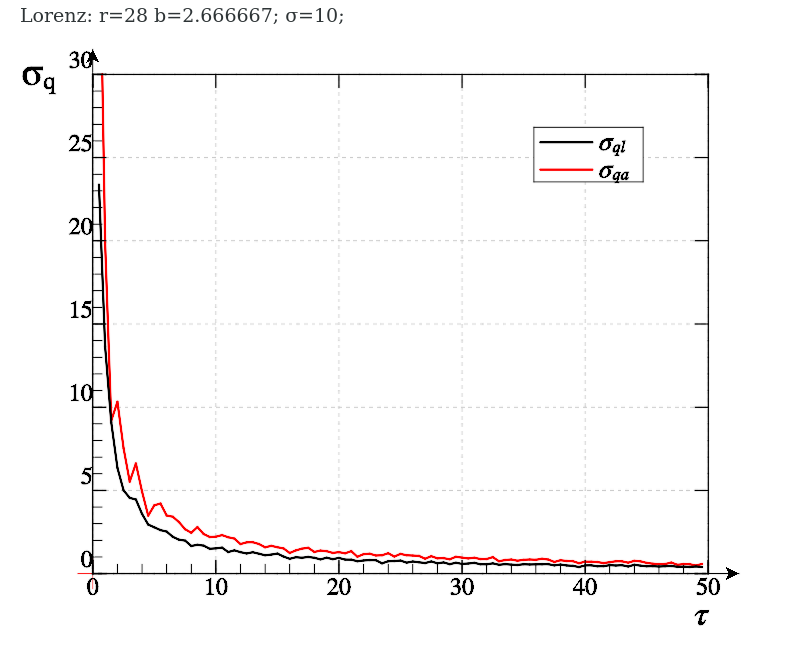
\includegraphics[width=0.49\textwidth]{p/cha/lor/lor_q_tau-p_tau_sd.png}
\end{center}
\caption{Залежності $ \sigma_{q} (a_q) $ і $ \sigma_{q} (\tau_q) $ для системи Лоренца, критерій $q_{y^2}$}
\label{atu:f:lor_qy2_tau}
\end{figure}


\begin{figure}[ht!]
\begin{center}
  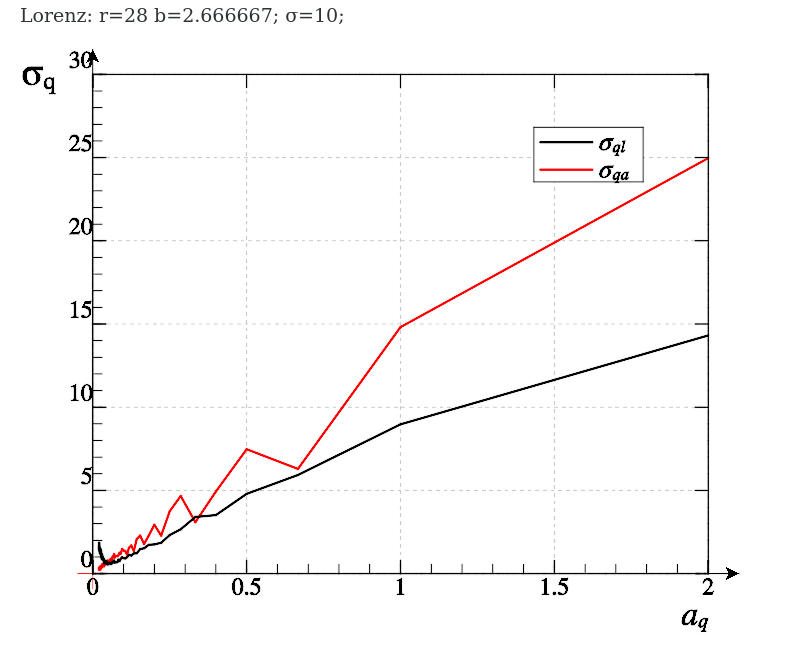
\includegraphics[width=0.49\textwidth]{p/cha/lor/lor_qx2_tau-p_aq_sd.png}
  \hfill
  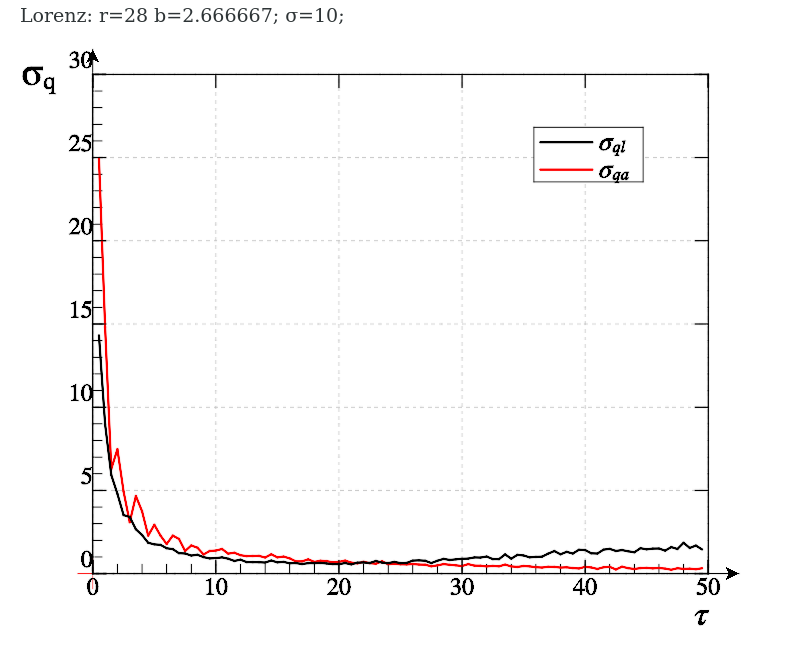
\includegraphics[width=0.49\textwidth]{p/cha/lor/lor_qx2_tau-p_tau_sd.png}
\end{center}
  \caption{Залежності $ \sigma_{q} (a_q) $ і $ \sigma_{q} (\tau_q) $ для системи Лоренца, критерій $q_{x^2}$}
\label{atu:f:lor_qx2_tau}
\end{figure}

Аналіз отриманих залежностей дозволяє зробити кілька
висновків. Перш за все, для даної системи результат усереднення
за допомогою значно більше витратного в реалізації
методу змінного середнього практично скрізь поступається
більш простому методу. Таким чином, при реалізації методів
ідентифікації в умовах з обмеженим ресурсами, наприклад на
микроконтроллерної платформі в реальному часі, немає сенсу
реалізовувати витратне ковзне середнє. Далі, сам вид
залежності виявився досить простим:
$ \sigma_q \sim q a_q $ або ж
$ \frac{\sigma_q \tau_q}{q} \approx \mathrm{const}$.

% }}}2


\subsection{Тестова задача ідентифікації для системи Лоренца}%{{{2

Відповідно до отриманих даних, і використовуючи
визначення~(\ref{atu:eq:po_t_sign}) і~(\ref{atu:eq:po_t_sin}),
%
визначимо тестові завдання наступним чином:
\[
  p(t) \in [20, 60],
\]
%
\begin{equation}
  r_o(t) = p_o(t) = p_0 +  U_{p} \sign \sin( \omega_{p} t ),
  \label{atu:eq:lor_po_t_sign}
\end{equation}
%
%
\begin{equation}
  r_o(t) = p_o(t) = p_0 +  U_{p} \sin( \omega_{p} t ),
  \label{atu:eq:lor_po_t_sin}
\end{equation}
%
де:
$p_0 = 37$, $U_p=12$, $\omega_p=0.09$.

В якості точки відліку розглянемо застосування вже розглянуто
в роботі~\cite{atu_phd_thesis}
метода, який використовує два УГПК і інтегратор для визначення динаміки одного агента,
який керує двома моделями, але з використянням кртерію, а не вихідних сигналів моделі тп об'єкту.
Для можливості застосування даного методу до системи
динамічного хаосу як об'єкт, так і моделі були доповнені блоками
оцінювання критерію
$ q_{x^2} $. Таким чином, згідно з ведений класифікації, метод
отримує позначення
``Fl2nlosdlcA.$q_{x^2}$''.

Перш за все, розглянемо процеси ідентифікації параметра
$ r $ системи Лоренца даним методом. Типові результати моделювання
наведені на рис.~(\ref{atu:f:lor_id_Fl2nlosdlcA_wp009}).

\begin{figure}[ht!]
  \centerline{
    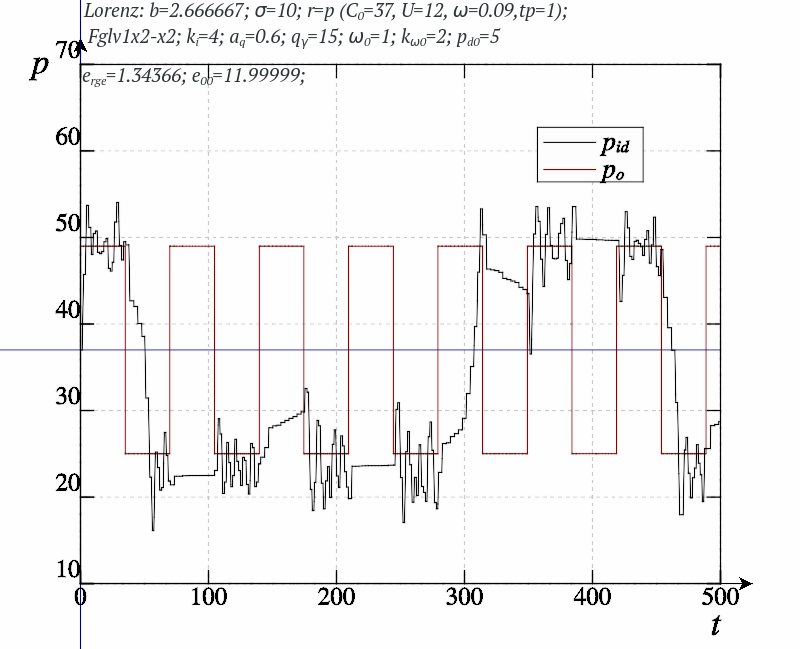
\includegraphics[width=0.49\textwidth]{p/cha/lor/Fl2nlosdlcA/Fl2nlosdlcA-p_xz_1_wp009.png}
    \hfill
    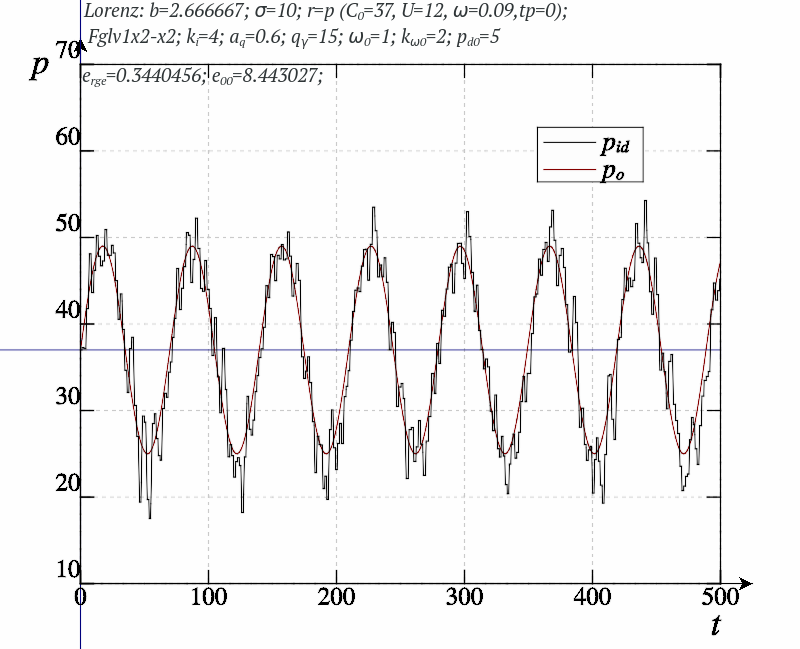
\includegraphics[width=0.49\textwidth]{p/cha/lor/Fl2nlosdlcA/Fl2nlosdlcA-p_xz_0_wp009.png}
  }
\caption{Процес ідентифікації параметра ``$ r $ '' системи Лоренца методом Fl2nlosdlcA.$q_{x^2} $ при умовах~(\ref{atu:eq:lor_po_t_sign}) і (\ref{atu:eq:lor_po_t_sin})}
\label{atu:f:lor_id_Fl2nlosdlcA_wp009}
\end{figure}

Як видно з графіків процесів ідентифікації, при заданих умовах
і при досить плавній зміні параметрів (\ref{atu:eq:lor_po_t_sin}) процес
ідентифікації призводить до позитивного результату. Якщо ж
значення параметра змінюються стрибкоподібно~(\ref{atu:eq:lor_po_t_sign}),
то процес пошуку порушується --- система просто не встигає
відреагувати на такі зміни. Спроби зменшити час реакції за
рахунок зміни відповідних параметрів ($ a_q $,
$ k_\omega $,
$ k_i $) призводять до повного порушення процесу пошуку. З іншого
боку, зменшення чутливості (збільшення $ q_\gamma $) дає можливість відновити працездатність процесу
ідентифікації ціною значного збільшення похибки.

Для перевірки тези про те, що в даному випадку грає роль саме
динаміка зміни
$ p_o (t) $, знизимо частоту
$ \omega_p $ до
$ 0.03 $ і проведемо моделювання при тих же значеннях всіх інших
параметрів. Результати наведені на рис.~\ref{atu:f:lor_id_Fl2nlosdlcA_003}.

\begin{figure}[ht!]
  \centerline{
    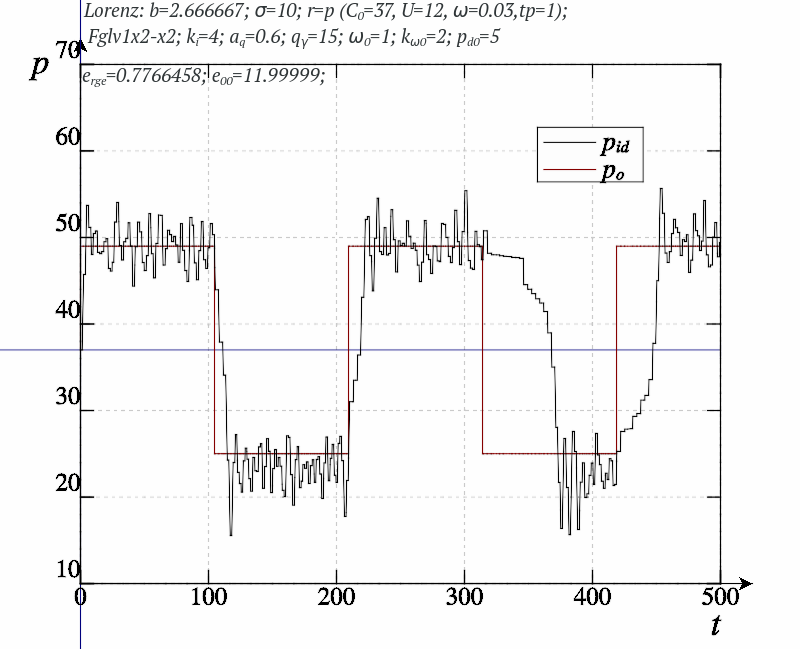
\includegraphics[width=0.49\textwidth]{p/cha/lor/Fl2nlosdlcA/Fl2nlosdlcA-p_xz_1_wp003.png}
    \hfill
    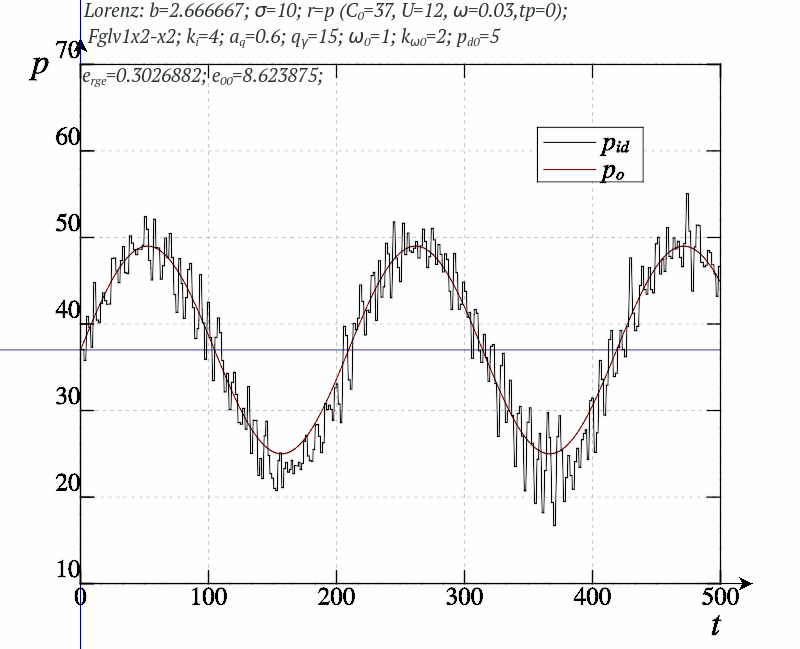
\includegraphics[width=0.49\textwidth]{p/cha/lor/Fl2nlosdlcA/Fl2nlosdlcA-p_xz_0_wp003.png}
  }
\caption{Процес ідентифікації параметра ``$ r $ '' системи Лоренца методом Fl2nlosdlcA.$q_{x^2} $ при $ \omega_p = 0.03 $}
  \label{atu:f:lor_id_Fl2nlosdlcA_003}
\end{figure}

Як і слід було очікувати, при меншому значенні
$ \omega_p $ обидва графіка підтверджують працездатність системи
ідентифікації.

Для оцінювання меж застосування методу з одним агентом і двома
моделями побудуємо залежності
$\overline{e}_{rge}(\omega_p)$~(рис.~\ref{atu:f:lor_Fl2nlosdlcA_e_omega_p}).

\begin{figure}[ht!]
  \centerline{
    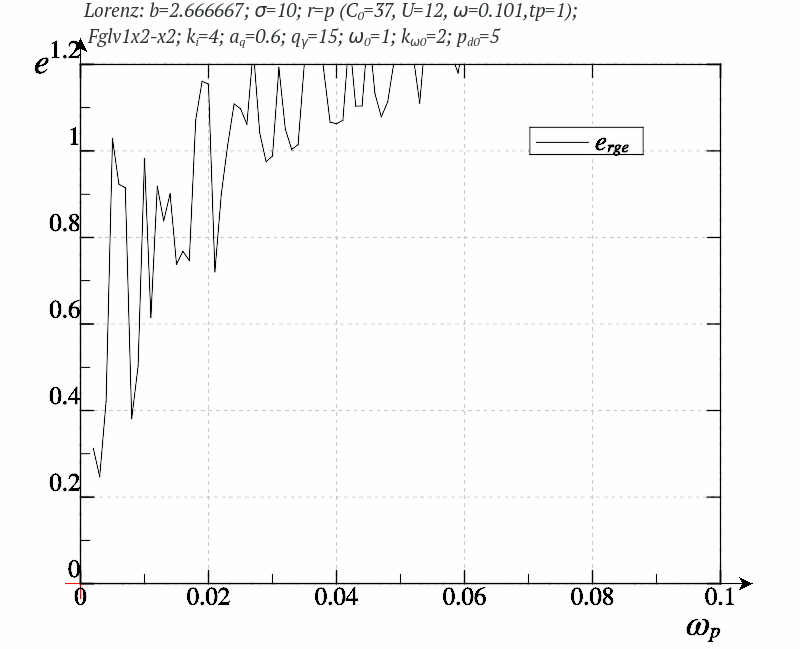
\includegraphics[width=0.49\textwidth]{p/cha/lor/Fl2nlosdlcA/Fl2nlosdlcA-p_omega_p_e_1.png}
    \hfill
    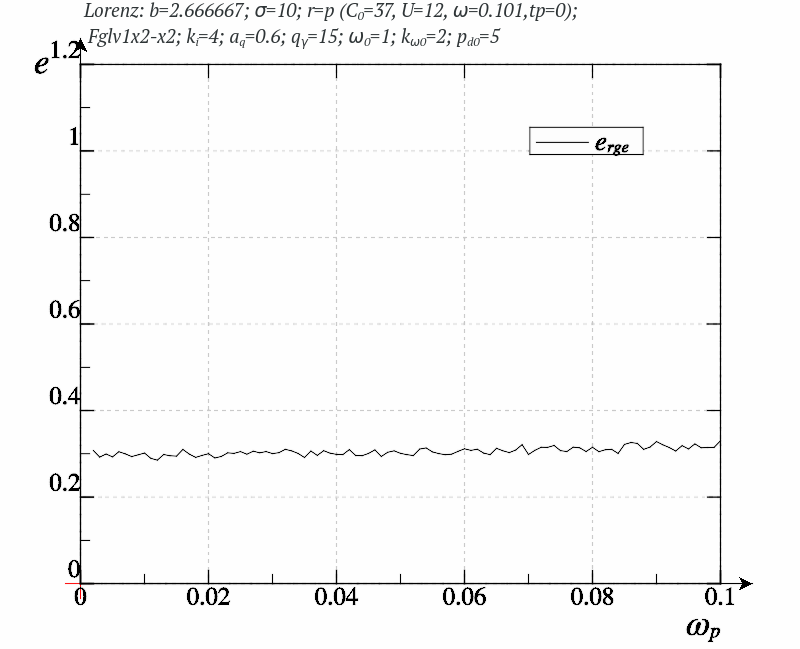
\includegraphics[width=0.49\textwidth]{p/cha/lor/Fl2nlosdlcA/Fl2nlosdlcA-p_omega_p_e_0.png}
  }
  \caption{Зависимости $\overline{e}_{rge}(\omega_p)$ при идентификации системы Лоренца методом Fl2nlosdlcA.$q_{x^2}$}
  \label{atu:f:lor_Fl2nlosdlcA_e_omega_p}
\end{figure}

Цілком очевидно, що розглянута система ідентифікації
має дуже обмежений діапазон застосовності за
умови~(\ref{atu:eq:lor_po_t_sign}). Умова~(\ref{atu:eq:lor_po_t_sin}) не накладає таких
жорстких обмежень. Однак, розглянувши цю ж залежність в іншому
масштабі~(рис.~\ref{atu:f:lor_Fl2nlosdlcA_e_omega_p_wide}), ми побачимо, що обмеження
все ж таки присутньє.

\begin{figure}[ht!]
  \centerline{
    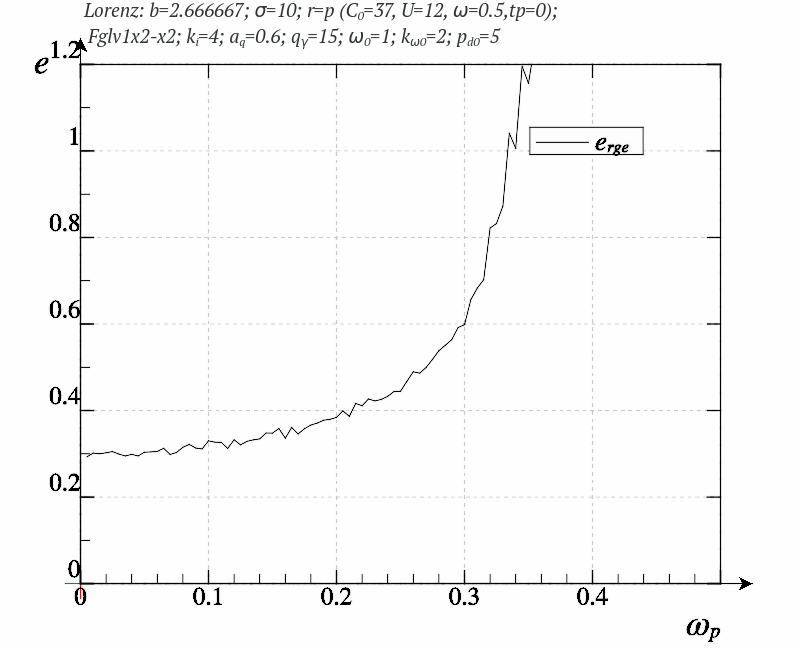
\includegraphics[width=0.49\textwidth]{p/cha/lor/Fl2nlosdlcA/Fl2nlosdlcA-p_omega_p_e_0_wide.png}
  }
\caption{Залежність $\overline{e}_{rge}(\omega_p) $ при ідентифікації системи Лоренца методом Fl2nlosdlcA.$q_{x^2} $}
\label{atu:f:lor_Fl2nlosdlcA_e_omega_p_wide}
\end{figure}

Так як основним недоліком розглянутого методу є обмежена
реакція на різку зміну параметра, то має сенс висунути
припущення, що використання в системі ідентифікації декількох
агентів, розподілених на просторі параметрів, може компенсувати
цей недолік.


Для порівняння були обрані три групи мультімодельніх методів
ідентіфікації~\cite{atu_ISDMCI2015,atu_asau26}:
ql3ruonAAF.$q_{x^2} $,
ql3ruonAAF.$q_{y^2} $ та
Fq3zlovnAAF.$q_{x^2} $.
Символи ``A '' в кожному з позначень~(див.~стор.~\pageref{atu:id_classification}) означають, що
перевіряється кілько способів визначення
$ p_\mathrm{id} $. Кількість агентів і спосіб їх угруповання (5.3) були
обрані однаковими для коректного порівняння різних походів.


На рис.~\ref{atu:f:lor_id_ql3ruonAAF.q_x2_sign} представлені результати
ідентифікації методом ql3ruonAAF.$q_{x^2} $, при цьому на лівому графіку зображено динаміку
переміщення кожної з рухливих моделей, а на правому --- 4 способи
визначення
$ p_{id} (t)$:
$ p_{gc} $,
$ p_{lc} $,
$ p_{ge} $ і
$ p_{le} $. В першу чергу, слід зазначити загальну працездатність
методів, і правильну динаміку кожної з моделей.


Порівнюючи результати різних способів визначення
$ p_{id} $ як візуально, так і чисельно, можна зробити висновок, що
гірші результати демонструє
$ p_{gc} $. Цього і слід було очікувати, так як це підхід, в першу
чергу, був призначений для методів ідентифікації користувачів
послуги якості для визначення
$ p_e $. Також, абсолютно очікувано, кращі результати
продемонстрував підхід
$ p_{qe} $. Також, при штучних обмеження
$ v_f = 0 $ і
$ q_\gamma = 0.1 $ були отримані величини, що характеризують якість
ідентифікації для нерухомих агентів:$ \overline{e}_{bc} = 9.85 $ і
$ \overline{e}_{be} = 7.09 $, що свідчить про виправданість як переміщення
агентів, так і використанні величин
$ p_e $ для визначення
$ p_{id} $.



\begin{figure}[ht!]
  \centerline{
    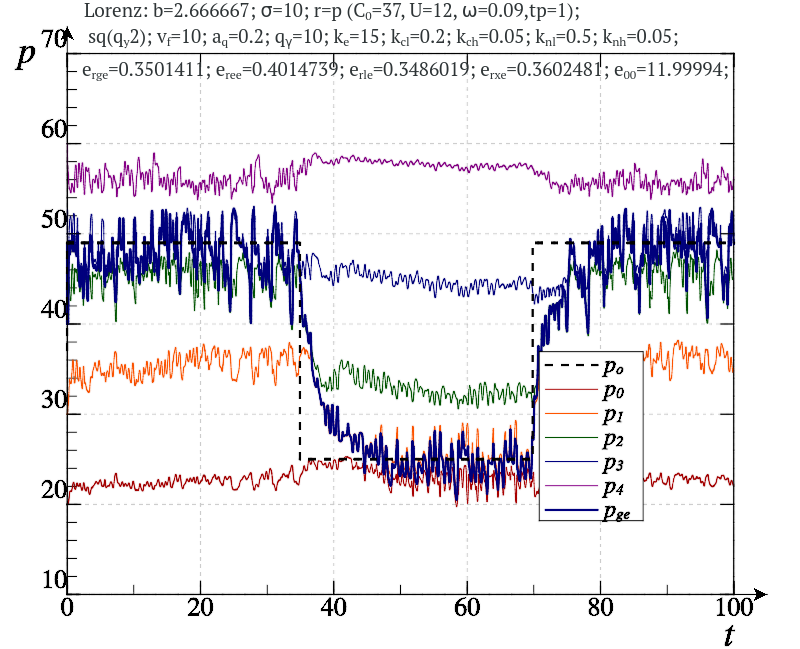
\includegraphics[width=0.49\textwidth]{p/cha/lor/ql3ruonAAF/lor_ql3ruonAAF_qy2-p_t_pi_sign.png}
    \hfill
    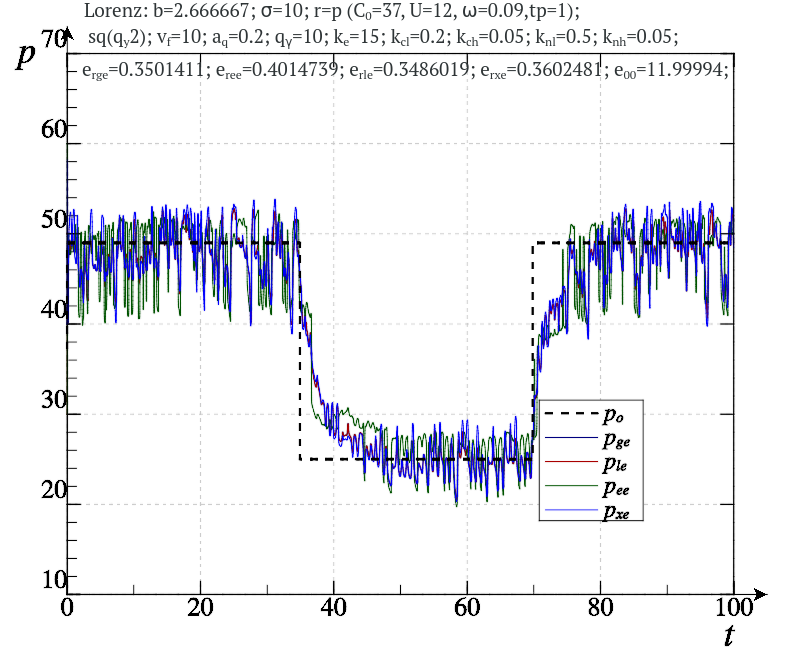
\includegraphics[width=0.49\textwidth]{p/cha/lor/ql3ruonAAF/lor_ql3ruonAAF_qy2-p_t_pz_sign.png}
  }
\caption{Процес ідентифікації параметра ``$r$ '' системи Лоренца методом ql3ruonAAF.$q_{x^2} $ за умови~(\ref{atu:eq:lor_po_t_sign})}
  \label{atu:f:lor_id_ql3ruonAAF.q_x2_sign}
\end{figure}


На рис.~\ref{atu:f:lor_id_ql3ruonAAF.q_x2_sin} представлені аналогічні результати,
але за умови плавнії зміни значення параметра об'єкта. Як і слід
було очікувати, як абсолютні, так і відносні значення помилок
ідентифікації в даному випадку помітно менше, при збереженні
загальної картини. При цьому
$\overline{e}_{bc}=7.80$
и
$\overline{e}_{be}=5.24$.


\begin{figure}[ht!]
  \centerline{
    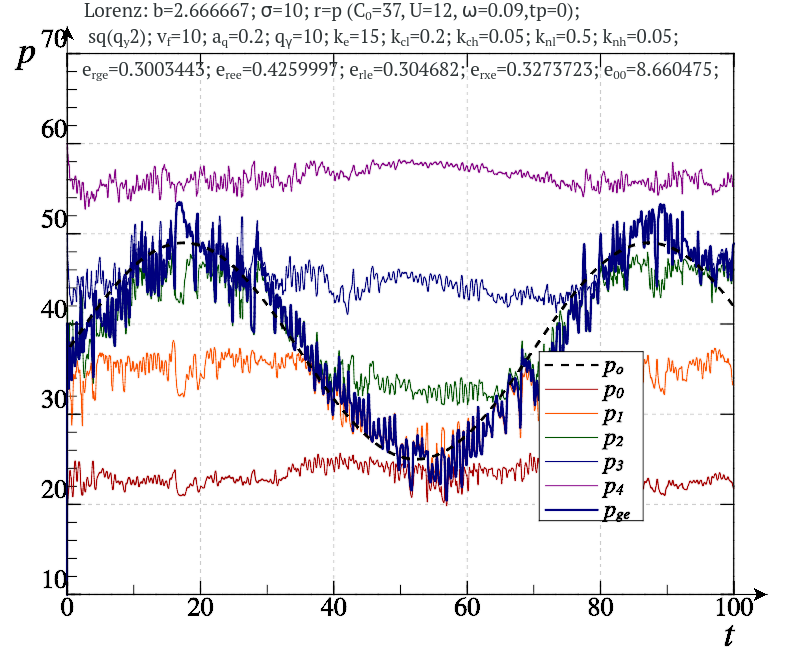
\includegraphics[width=0.49\textwidth]{p/cha/lor/ql3ruonAAF/lor_ql3ruonAAF_qy2-p_t_pi_sin.png}
    \hfill
    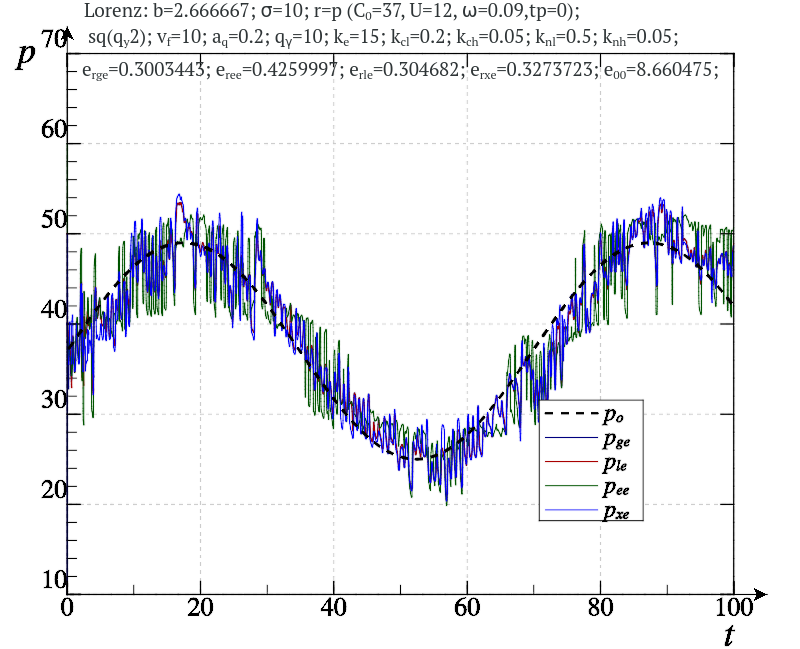
\includegraphics[width=0.49\textwidth]{p/cha/lor/ql3ruonAAF/lor_ql3ruonAAF_qy2-p_t_pz_sin.png}
  }
\caption{Процес ідентифікації параметра ``$ r $ '' системи Лоренца методом ql3ruonAAF.$q_{x^2} $ за умови~(\ref{atu:eq:lor_po_t_sin})}
\label{atu:f:lor_id_ql3ruonAAF.q_x2_sin}
\end{figure}


На рис.~\ref{atu:f:lor_id_ql3ruonAAF.q_y2_sign} представлені результати отримані
методом ql3ruonAAF.$q_{y^2}$, що відрізняється від попереднього тільки видом
використаного критерію. При цьому
$\overline{e}_{bc}=10.85$
та
$\overline{e}_{be}=7.73$.

\begin{figure}[ht!]
  \centerline{
    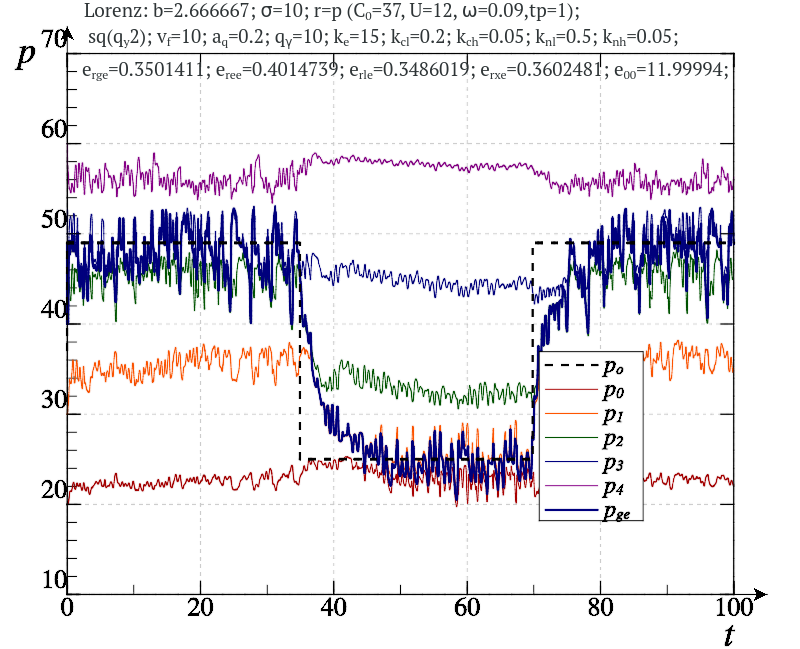
\includegraphics[width=0.49\textwidth]{p/cha/lor/ql3ruonAAF/lor_ql3ruonAAF_qy2-p_t_pi_sign.png}
    \hfill
    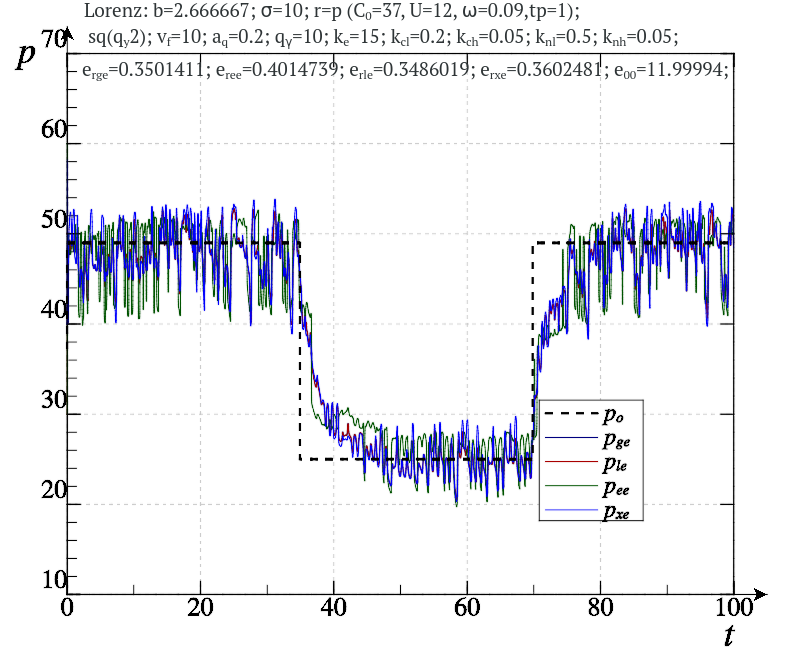
\includegraphics[width=0.49\textwidth]{p/cha/lor/ql3ruonAAF/lor_ql3ruonAAF_qy2-p_t_pz_sign.png}
  }
\caption{Процес ідентифікації параметра ``$ r $ '' системи Лоренца методом ql3ruonAAF.$q_{y^2}$ за умови~(\ref{atu:eq:lor_po_t_sign})}
  \label{atu:f:lor_id_ql3ruonAAF.q_y2_sign}
\end{figure}


На рис.~\ref{atu:f:lor_id_ql3ruonAAF.q_y2_sin} представлені аналогічні результати,
тільки за умови (\ref{atu:eq:lor_po_t_sin}). При цьому
$\overline{e}_{bc}=8.09$
та
$\overline{e}_{be}=5.46$.


\begin{figure}[ht!]
  \centerline{
    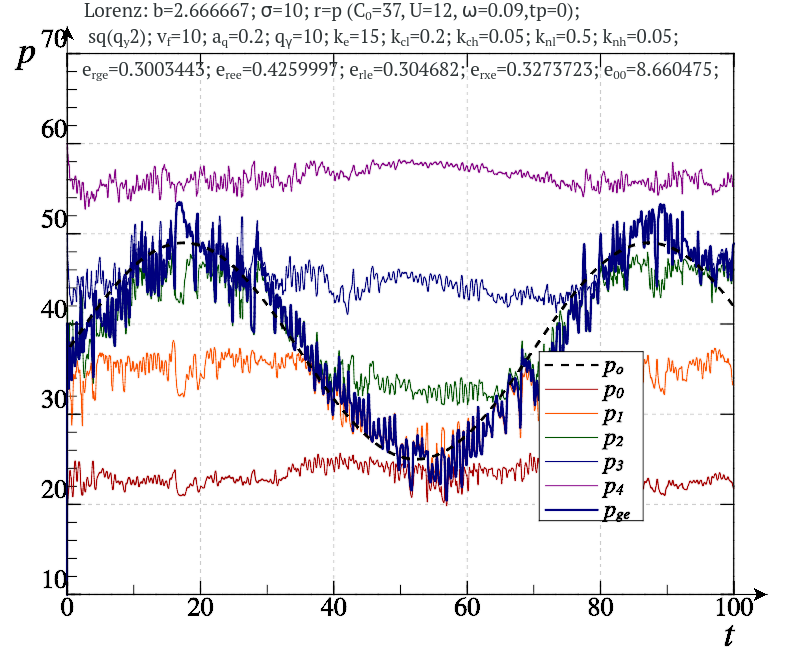
\includegraphics[width=0.49\textwidth]{p/cha/lor/ql3ruonAAF/lor_ql3ruonAAF_qy2-p_t_pi_sin.png}
    \hfill
    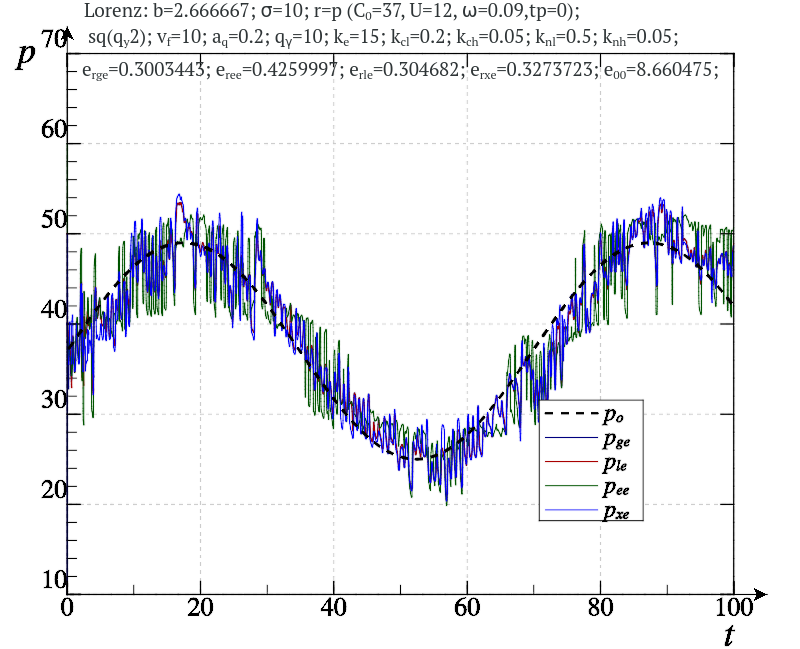
\includegraphics[width=0.49\textwidth]{p/cha/lor/ql3ruonAAF/lor_ql3ruonAAF_qy2-p_t_pz_sin.png}
  }
\caption{Процес ідентифікації параметра ``$ r $ '' системи Лоренца методом ql3ruonAAF.$q_{x^2} $ за умови~(\ref{atu:eq:lor_po_t_sin})}
  \label{atu:f:lor_id_ql3ruonAAF.q_y2_sin}
\end{figure}

Також важливим результатом є той факт, що, в порівнянні з
одноагентним методом, система ідентифікації не втрачає
працездатності при різких змінах параметра. Залежності
$ \overline{e}_{rge} (\omega_p) $ для даної групи методів наведені на
рис.~\ref{atu:f:lor_ql3ruonAAF_e_omega_p}.


\begin{figure}[ht!]
  \centerline{
    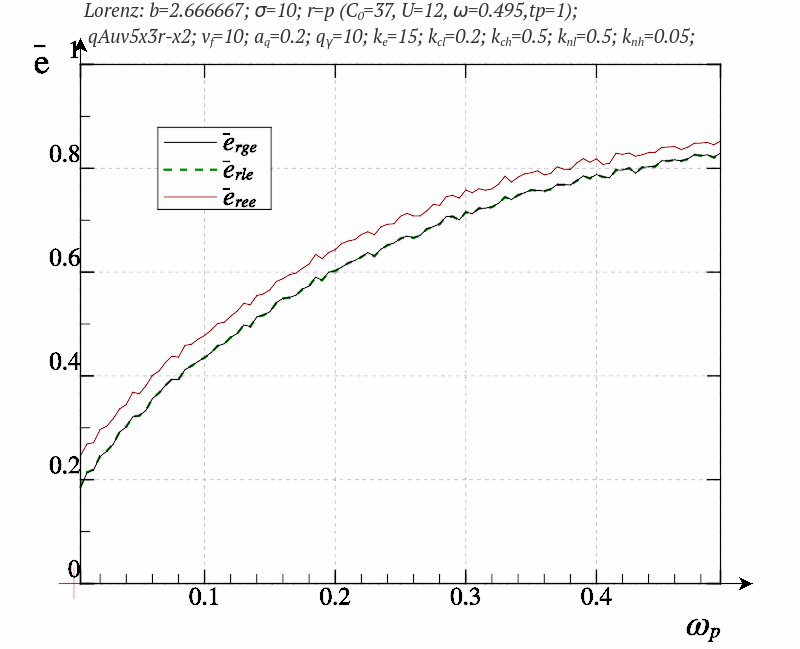
\includegraphics[width=0.49\textwidth]{p/cha/lor/ql3ruonAAF/lor_ql3ruonAAF_qx2-p_omega_p_e_sign.png}
    \hfill
    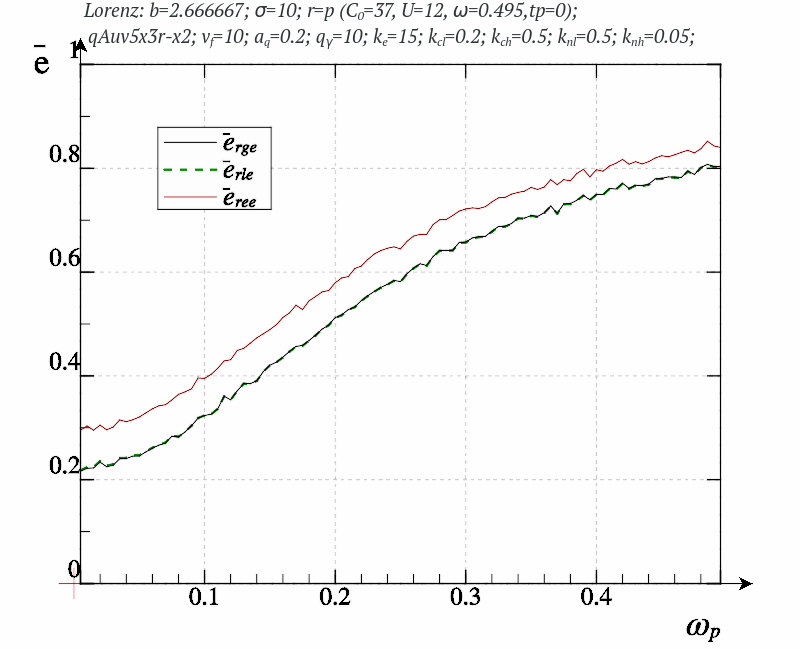
\includegraphics[width=0.49\textwidth]{p/cha/lor/ql3ruonAAF/lor_ql3ruonAAF_qx2-p_omega_p_e_sin.png}
  }
\caption{Залежності $ \overline{e}_{rge} (\omega_p) $ при ідентифікації системи Лоренца методом ql3ruonAAF.$q_{x^2} $}
\label{atu:f:lor_ql3ruonAAF_e_omega_p}
\end{figure}

Порівнювати отримані залежності з аналогічними для
одноагентого методу (рис.~\ref{atu:f:lor_Fl2nlosdlcA_e_omega_p}), можна з
упевненістю констатувати, що застосування мультиагентного
підходу тут повністю виправдано. По-перше, допустимий діапазон
$ \omega_p $ розширюється як мінімум на порядок. З іншого боку, в цьому
випадку немає принципової різниці між умовами~(\ref{atu:eq:lor_po_t_sign})
і (\ref{atu:eq:lor_po_t_sin}), що також є безперечною перевагою.




Порівнюючи результати, представлені на
рис.~\ref{atu:f:lor_id_ql3ruonAAF.q_x2_sign} -- \ref{atu:f:lor_id_ql3ruonAAF.q_y2_sin} можна зробити
наступні висновки:

\begin{itemize}

  \item
   Динаміка систем ідентифікації при використанні критеріїв $ q_{x^2} $ і $ q_{y^2} $ практично збігається.

  \item
    Застосування критерію
    $ q_{y^2} $ в даному конкретному випадку дозволяє меншу похибку
    ідентифікації, але на настільки, щоб можна було говорити про
    істотну різницю.

  \item
    У всіх розглянутих випадках виправданими були і застосування
    декількох агентів, і їх зміщення в процесі пошуку, і визначення
    за допомогою
    $p_e$ кожного з агентів.

\end{itemize}

Розглянемо процес ідентифікації цієї ж системи, при тих же
умовах, але сімейством методів, заснованих на застосуванні
функції якості, а саме
Fq3zlovnAAF.$q_{x^2}$

Процес ідентифікації за умови~(\ref{atu:eq:lor_po_t_sign}) представлений
на рис.~\ref{atu:f:lor_id_Fq3zlovnAAF.q_x2_sign}. В першу чергу слід відзначити
велику рухливість агентів, аж до штучного обмеження рухливості
здебільшого моделей. З одного боку, це дещо зменшує швидкодію
системи при різких змінах параметра, з іншого --- забезпечує
достатню зміщення ``далеких'' агентів, що, в якійсь мірі,
компенсує можливі похибки в налаштуванні системи. Величина
$ \overline{e}_{bc} = 10.84 $ має приблизно таке ж значення, як і попередніх
випадках, а
$ \overline{e}_{be} $ в даних умовах не може бути застосована.

\begin{figure}[ht!]
  \centerline{
    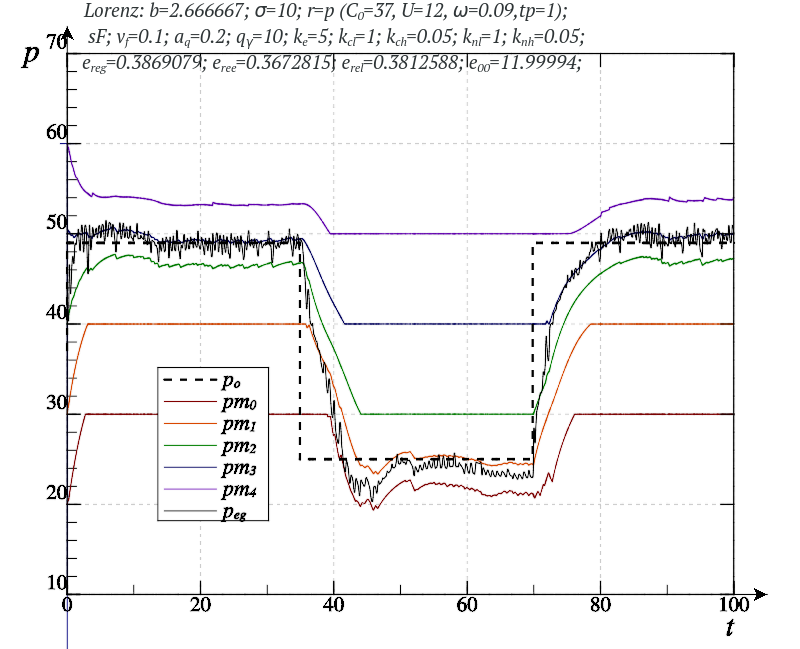
\includegraphics[width=0.49\textwidth]{p/cha/lor/Fq3zlovnAAF/lor_Fq3zlovnAAF_qx2-pl_n_sign.png}
    \hfill
    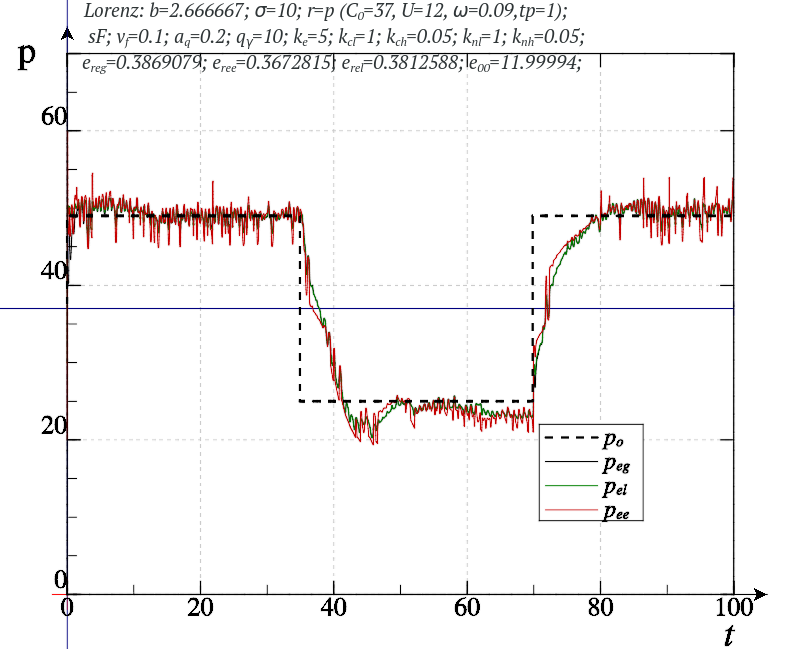
\includegraphics[width=0.49\textwidth]{p/cha/lor/Fq3zlovnAAF/lor_Fq3zlovnAAF_qx2-p_p_sign.png}
  }
\caption{Процес ідентифікації параметра ``$ r $ '' системи Лоренца методом Fq3zlovnAAF.$q_{x^2} $ за умови~(\ref{atu:eq:lor_po_t_sign})}
\label{atu:f:lor_id_Fq3zlovnAAF.q_x2_sign}
\end{figure}

На рис.~\ref{atu:f:lor_id_Fq3zlovnAAF.q_x2_sin} представлено процес ідентифікації за
умови~(\ref{atu:eq:lor_po_t_sin}). Величина
$ \overline{e}_{bc} = 7.95 $ не вибивається із загального ряду, і загальна
картина має очікуваний вид.

\begin{figure}[ht!]
  \centerline{
    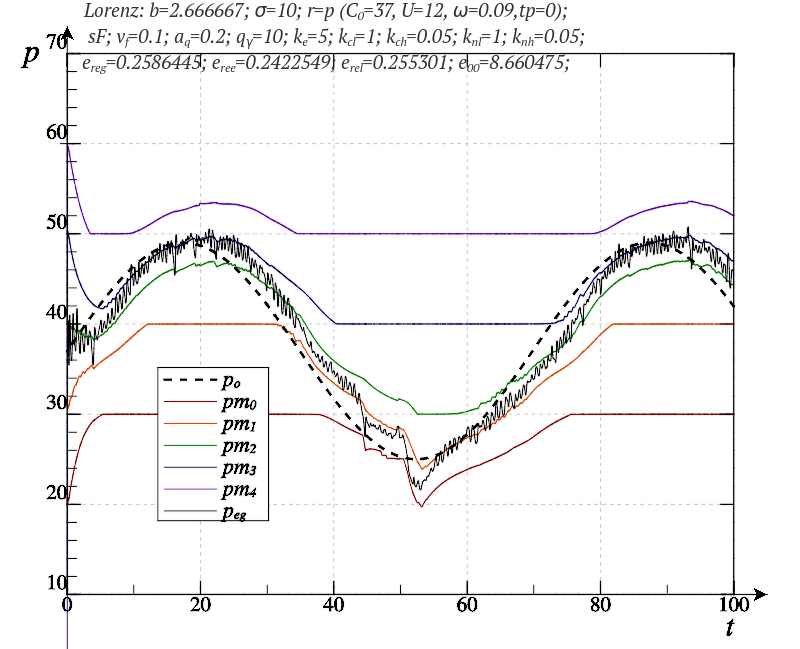
\includegraphics[width=0.49\textwidth]{p/cha/lor/Fq3zlovnAAF/lor_Fq3zlovnAAF_qx2-pl_n_sin.png}
    \hfill
    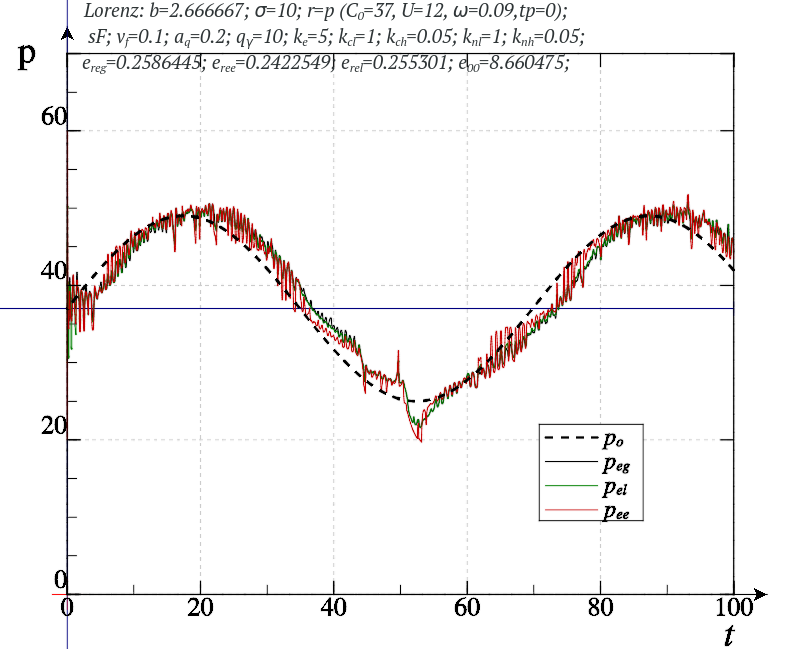
\includegraphics[width=0.49\textwidth]{p/cha/lor/Fq3zlovnAAF/lor_Fq3zlovnAAF_qx2-p_p_sin.png}
  }
\caption{Процес ідентифікації параметра ``$ r $ '' системи Лоренца методом Fq3zlovnAAF.$q_{x^2} $ за умови~(\ref{atu:eq:lor_po_t_sin})}
\label{atu:f:lor_id_Fq3zlovnAAF.q_x2_sin}
\end{figure}

Також слід зазначити, що даний метод, аналогічно попередньому,
проявляє працездатність при різких змінах параметра. Побудуємо
залежності
$\overline{e}_{rge}(\omega_p)$ (рис.~\ref{atu:f:lor_Fq3zlovnAAF_e_omega_p}).


\begin{figure}[ht!]
  \centerline{
    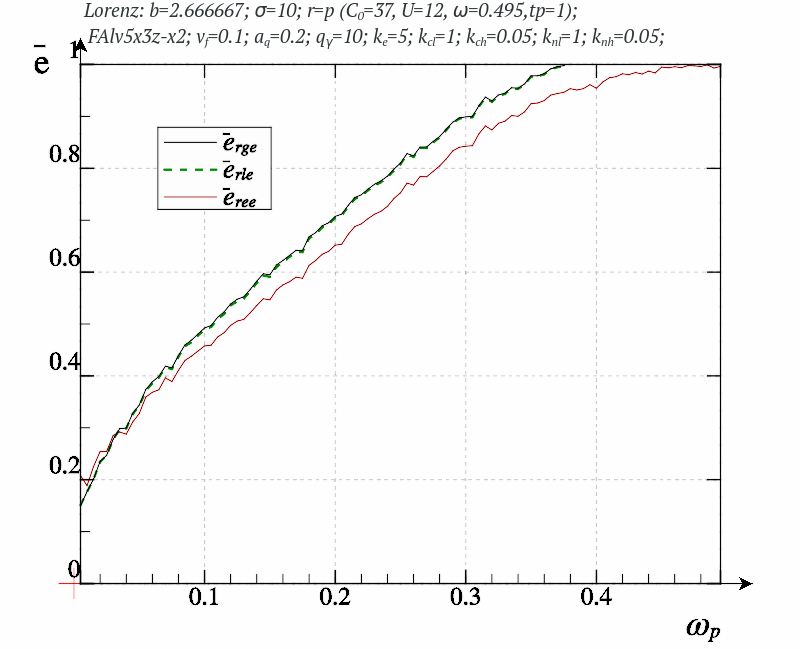
\includegraphics[width=0.49\textwidth]{p/cha/lor/Fq3zlovnAAF/lor_Fq3zlovnAAF_qx2-p_omega_p_e_sign.png}
    \hfill
    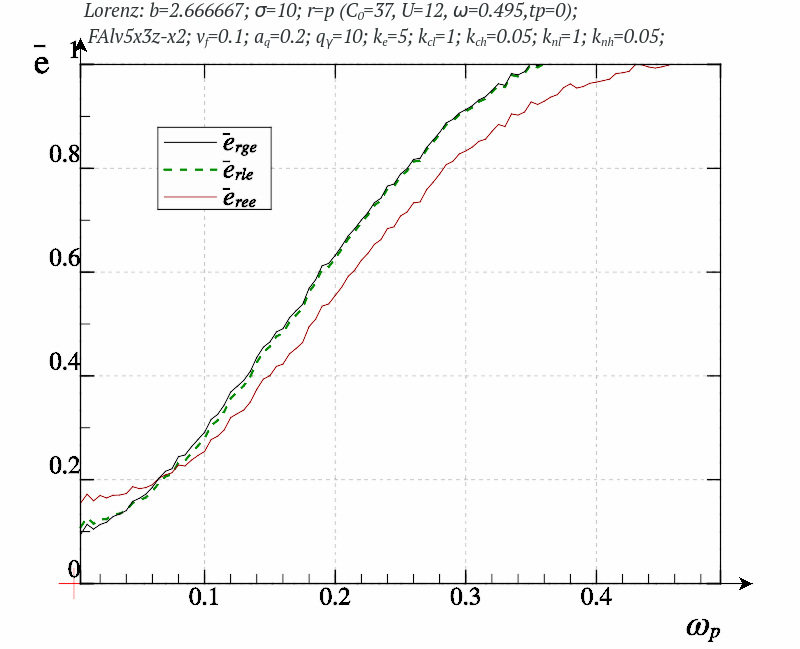
\includegraphics[width=0.49\textwidth]{p/cha/lor/Fq3zlovnAAF/lor_Fq3zlovnAAF_qx2-p_omega_p_e_sin.png}
  }
\caption{Залежності $ \overline{e}_{rge} (\omega_p) $ при ідентифікації системи Лоренца методом Fq3zlovnAAF.$q_{x^2} $}
\label{atu:f:lor_Fq3zlovnAAF_e_omega_p}
\end{figure}

Вид цих залежностей аналогічний таким для попереднього методу,
хоча робочий діапазон по
$ \omega_p $ незначно меньше. Таким чином, застосування мультімодельного
підходу виправдано, принаймні з цієї точки зору, незалежно
від того, яку величину,
$ q $ або
$ F $ використовують агенти для визначення
$ p_e $.

% }}}2


% ----------------------------------------- id_params -------------------------------

\subsection{Вплив параметрів системи ідентифікації на похибку ідентифікації для системи Лоренца} % {{{2

Розглянемо вплив параметрів системи ідентифікації на процес
ідентифікації і, отже, на її якість~\cite{atu_ISDMCI2014}. Для цього будемо
варіювати кожен з істотних параметрів і будувати залежно
$ \overline{e} $ для кожного з розглянутих методів.

В першу чергу розглянемо вплив параметра
$a_q$, що визначає характерний час усереднення.

На рис.~\ref{atu:f:lor_a_q_ql3ruonAAF.q_x2} представлені залежності усереднених
помилок ідентифікації системи Лоренца від
$ a_q $ при використанні методу
ql3ruonAAF.$q_{x^2}$.
Досить очевидно, що форма кривих з явним екстремумів обумовлена
впливами протиборчих факторів. При великих значеннях
$a_q$, і, отже, малу хвилю усереднення
$ \tau_q $, занадто сильно вплив хаотичної динаміки, що б можна було
б проводити успішну ідентифікацію. З іншого боку, при занадто
малих значеннях
$a_q$, час оцінювання критерію настільки велик, що система
ідентифікації не встигає відслідковувати зміну параметра. Ця
теза підтверджується тим фактом, що при більш плавній зміні
параметра (\ref{atu:eq:lor_po_t_sin}) мінімум помилок досягається при
менших значеннях
$a_q$.

\begin{figure}[ht!]
  \centerline{
    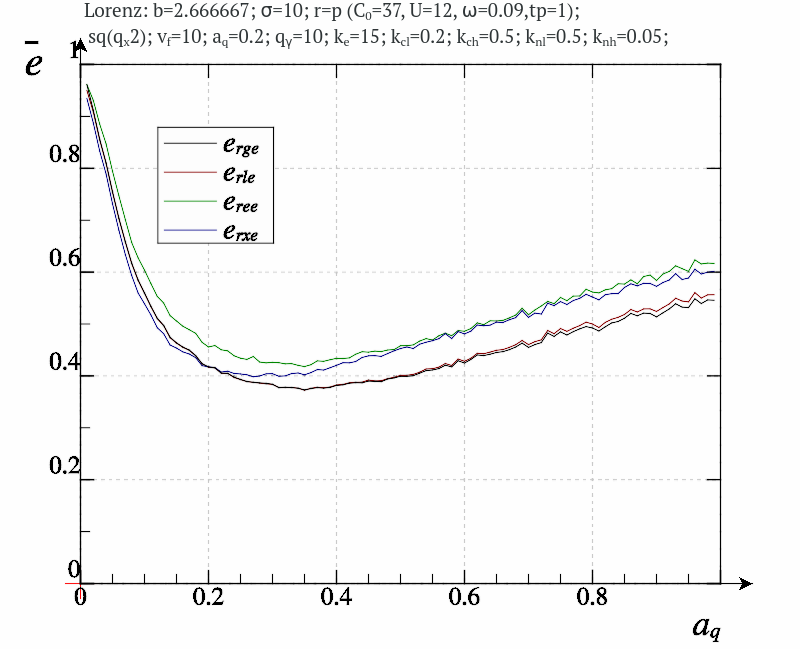
\includegraphics[width=0.49\textwidth]{p/cha/lor/ql3ruonAAF/lor_ql3ruonAAF_qx2-p_a_q_e_sign.png}
    \hfill
    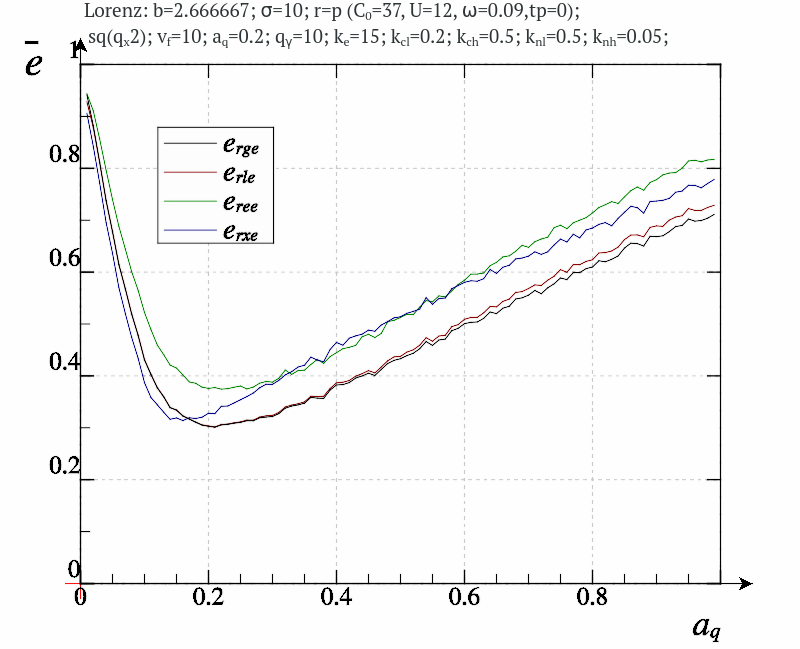
\includegraphics[width=0.49\textwidth]{p/cha/lor/ql3ruonAAF/lor_ql3ruonAAF_qx2-p_a_q_e_sin.png}
  }
  \caption{Залежності $ \overline{e}_{r *} (a_q) $ при ідентифікації системи Лоренца методом ql3ruonAAF.$q_{x^2} $ при~(\ref{atu:eq:lor_po_t_sign}) і (\ref{atu:eq:lor_po_t_sin})}
  \label{atu:f:lor_a_q_ql3ruonAAF.q_x2}
\end{figure}


На рис.~\ref{atu:f:lor_a_q_ql3ruonAAF.q_y2} представлені залежності усереднених
помилок ідентифікації системи Лоренца при використанні методу
ql3ruonAAF.$q_{y^2} $. Тут ситуація істотно змінюється але порівняно з
попереднім випадком. Положення екстремумів практично не
змінилися, але при великих значеннях
$ a_q $ починає спостерігатися повне порушення процесу
пошуку. Таким чином, незважаючи на те, що в найкращих умовах
критерій
$ q_{y^2} $ забезпечує меншу похибку ідентифікації, діапазон його
застосування менше. З урахуванням того, момент порушення пошуку
залежить і від форми
$ p_o (t) $, а вона в реальних задачах заздалегідь не відома,
використання цього критерію може не бути виправданим.

\begin{figure}[ht!]
  \centerline{
    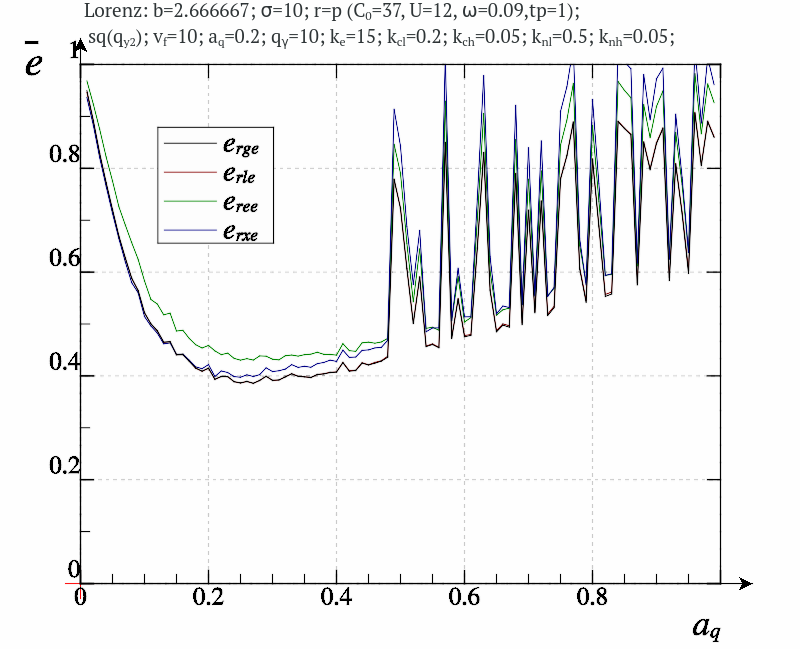
\includegraphics[width=0.49\textwidth]{p/cha/lor/ql3ruonAAF/lor_ql3ruonAAF_qy2-p_a_q_e_sign.png}
    \hfill
    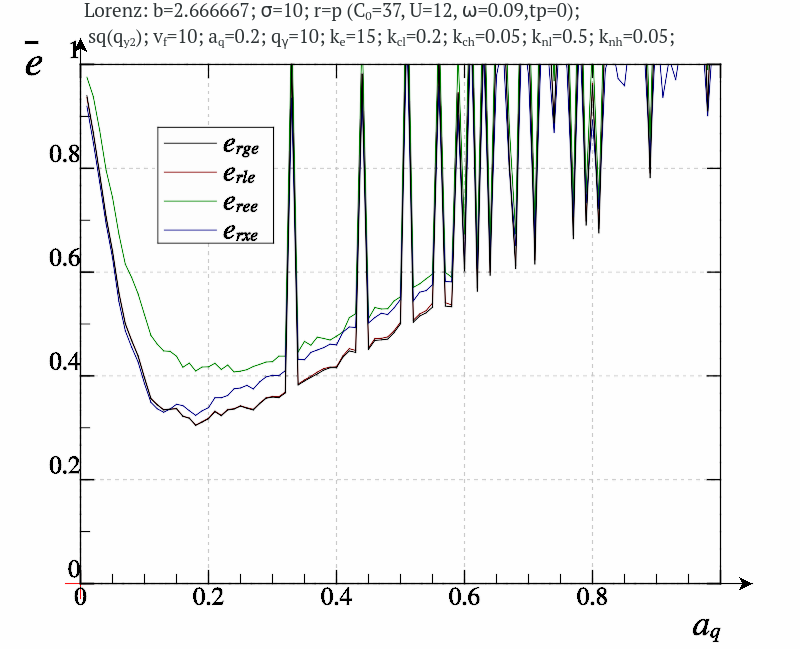
\includegraphics[width=0.49\textwidth]{p/cha/lor/ql3ruonAAF/lor_ql3ruonAAF_qy2-p_a_q_e_sin.png}
  }
\caption{Залежності $ \overline{e}_{r *} (a_q) $ при ідентифікації системи Лоренца методом ql3ruonAAF.$q_{y^2} $ при~(\ref{atu:eq:lor_po_t_sign}) і (\ref{atu:eq:lor_po_t_sin})}
  \label{atu:f:lor_a_q_ql3ruonAAF.q_y2}
\end{figure}


На рис.~\ref{atu:f:lor_a_q_Fq3zlovnAAF.q_x2} представлені залежності усереднених
помилок ідентифікації системи Лоренца при використанні методу
Fq3zlovnAAF.$q_{x^2}$.
Як характер залежностей, так і положення екстремумів аналогічні
нагоди при використанні методу
ql3ruonAAF.$q_{x^2}$,
хоча певні відмінності спостерігаються. Проте, можна зробити
висновок, що як оптимальні значення величини
$a_q$, так і діапазон застосовності в першу чергу визначається
критерієм і динамікою зміни параметра, і вже в другу чергу ---
конкретним методом.


\begin{figure}[ht!]
  \centerline{
    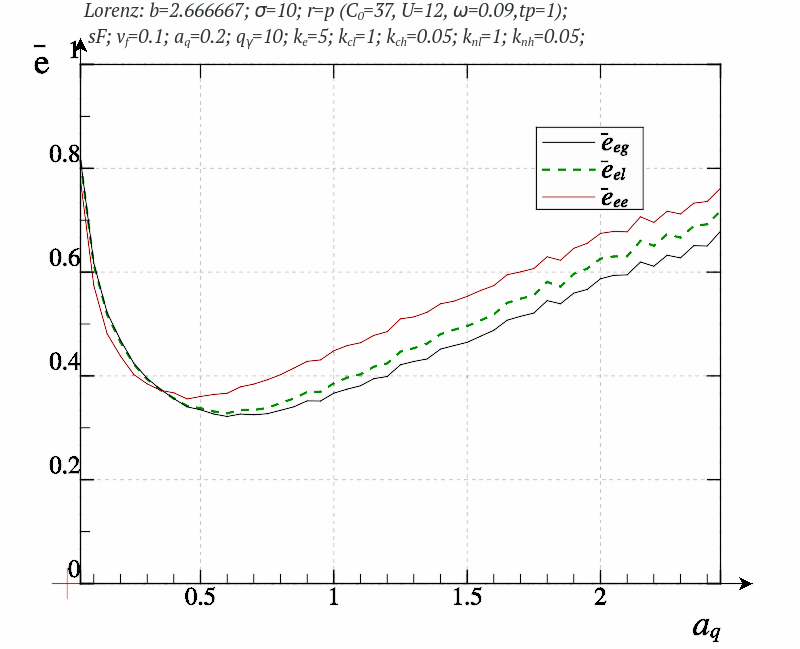
\includegraphics[width=0.49\textwidth]{p/cha/lor/Fq3zlovnAAF/lor_Fq3zlovnAAF_qx2-p_a_q_e_sign.png}
    \hfill
    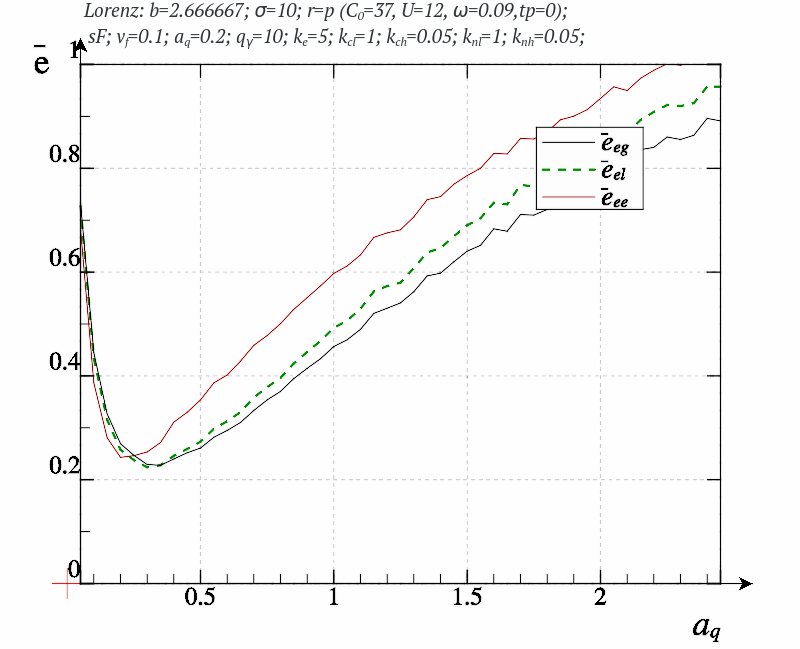
\includegraphics[width=0.49\textwidth]{p/cha/lor/Fq3zlovnAAF/lor_Fq3zlovnAAF_qx2-p_a_q_e_sin.png}
  }
\caption{Залежності $ \overline{e}_{r *} (a_q) $ при ідентифікації системи Лоренца методом Fq3zlovnAAF.$q_{x^2} $ при~(\ref{atu:eq:lor_po_t_sign}) і (\ref{atu:eq:lor_po_t_sin})}
\label{atu:f:lor_a_q_Fq3zlovnAAF.q_x2}
\end{figure}


Наступний важливий параметр - масштаб функції якості
$ q_\gamma $. В першу чергу він повинен впливати на методи, які
використовують величину
$ F $ в процесі пошуку. З іншого боку, методи, які використовують
тільки критерій для визначення
$ p_e $, теж використовують
$ q_\gamma $ в процесі визначення
$ p_\mathrm{id} $.

На рис.~\ref{atu:f:lor_qg_ql3ruonAAF.q_x2} представлені залежності усереднених
помилок ідентифікації системи Лоренца від
$ q_\gamma $ при використанні методу ql3ruonAAF.
$ q_{x^2} $. Як і передбачалося, залежно досить слабкі, за винятком
$ \overline{e}_{rge} $, для якої великі величини масштабу позначають малу
чутливість, і отже, надмірний вплив агентів, розташованих далеко
від шуканого значення параметра. Самі стійко хороші результати
демонструє
$ p_{qe} $.

\begin{figure}[ht!]
  \centerline{
    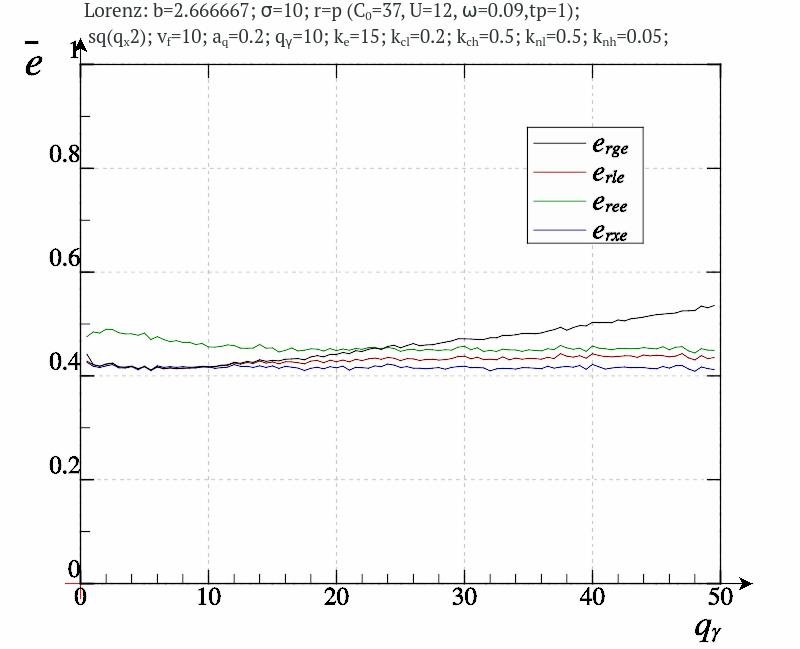
\includegraphics[width=0.49\textwidth]{p/cha/lor/ql3ruonAAF/lor_ql3ruonAAF_qx2-p_qgamma_e_sign.png}
    \hfill
    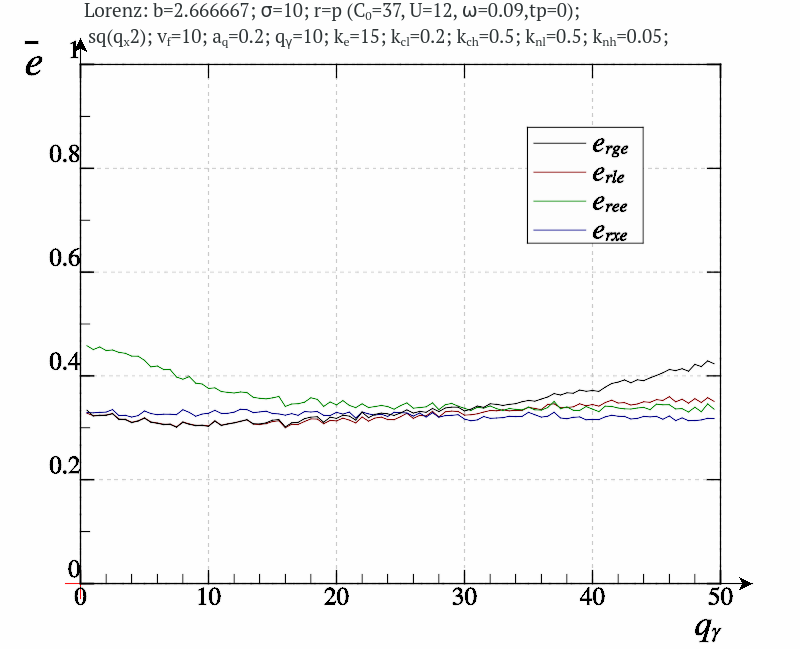
\includegraphics[width=0.49\textwidth]{p/cha/lor/ql3ruonAAF/lor_ql3ruonAAF_qx2-p_qgamma_e_sin.png}
  }
\caption{Залежності $ \overline{e}_{r *} (q_\gamma) $ при ідентифікації системи Лоренца методом ql3ruonAAF.$q_{x^2} $ при~(\ref{atu:eq:lor_po_t_sign}) і (\ref{atu:eq:lor_po_t_sin})}
\label{atu:f:lor_qg_ql3ruonAAF.q_x2}
\end{figure}



На рис.~\ref{atu:f:lor_qg_ql3ruonAAF.q_y2} представлені залежності усереднених
помилок ідентифікації системи Лоренца від
$ q_\gamma $ при використанні методу
ql3ruonAAF.$q_{y^2}$.
Тут результати аналогічні попередньому випадку. Однак, даний
підхід виявився більш чутливим до занижених значень $ q_\gamma $.

\begin{figure}[ht!]
  \centerline{
    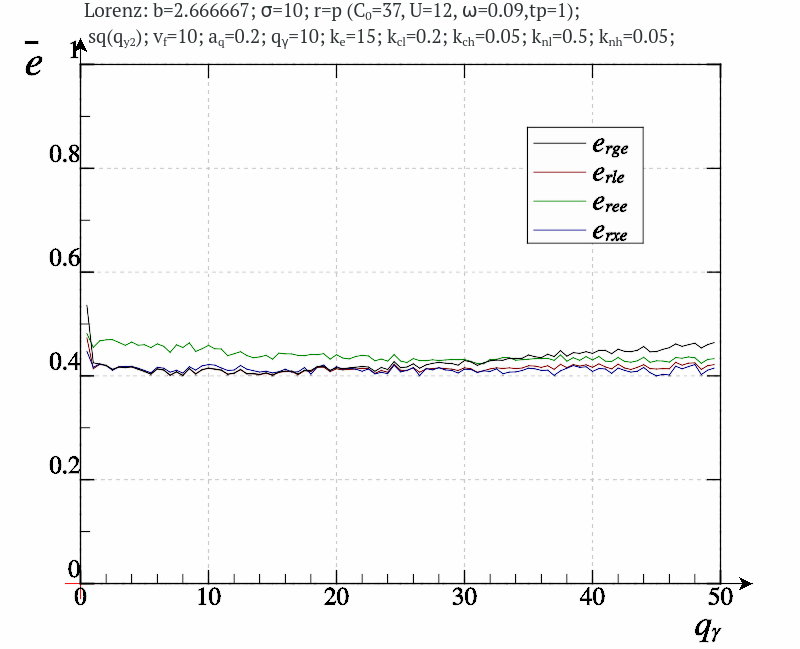
\includegraphics[width=0.49\textwidth]{p/cha/lor/ql3ruonAAF/lor_ql3ruonAAF_qy2-p_qgamma_e_sign.png}
    \hfill
    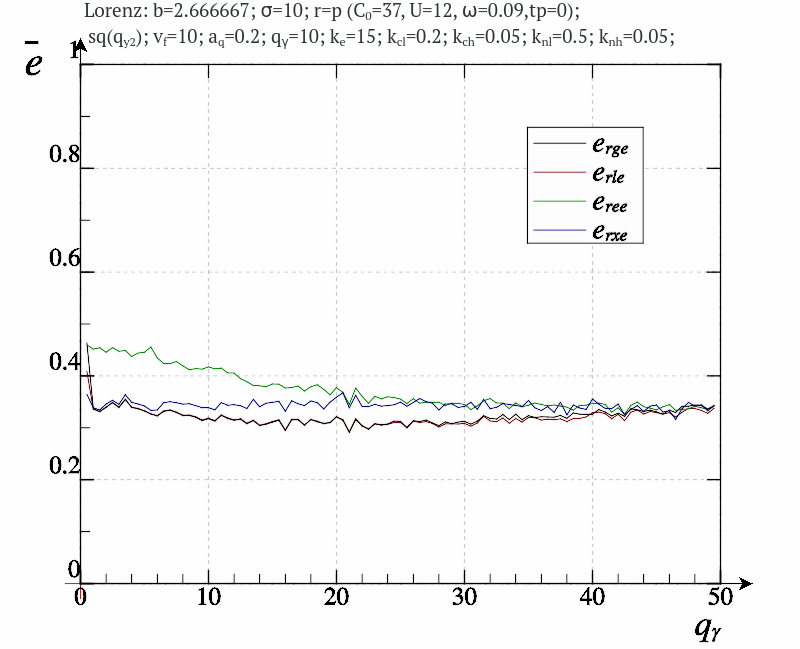
\includegraphics[width=0.49\textwidth]{p/cha/lor/ql3ruonAAF/lor_ql3ruonAAF_qy2-p_qgamma_e_sin.png}
  }
\caption{Залежності $ \overline{e}_{r *} (q_\gamma) $ при ідентифікації системи Лоренца методом ql3ruonAAF.$q_{y^2} $ при~(\ref{atu:eq:lor_po_t_sign}) і (\ref{atu:eq:lor_po_t_sin})}
  \label{atu:f:lor_qg_ql3ruonAAF.q_y2}
\end{figure}


На рис.~\ref{atu:f:lor_qg_Fq3zlovnAAF.q_x2} представлені залежності усереднених
помилок ідентифікації системи Лоренца від
$ q_\gamma $ при використанні методу
FAlv.3z.$q_{x^2}$.
У цьому випадку залежно сильно відрізняються від двох
попередніх випадків. Так як цей метод безпосередньо
використовують функцію якості для визначення
$ p_e $ кожним агентом, то залежність має явний екстремальний
характер. При малих значеннях
$ q_\gamma $ чутливість надлишкова, і процес пошуку порушується. При
великих - недостатня, і крім надлишкового впливу ``далеких''
агентів також знижується швидкість і точність пошуку. Вплив
``далеких'' агентів ігнорується при використанні
$ p_{le} $ і
$ p_{qe} $, проте, в ціх методах зменьщується точність при перемиканні
між кращими агентами.


\begin{figure}[ht!]
  \centerline{
    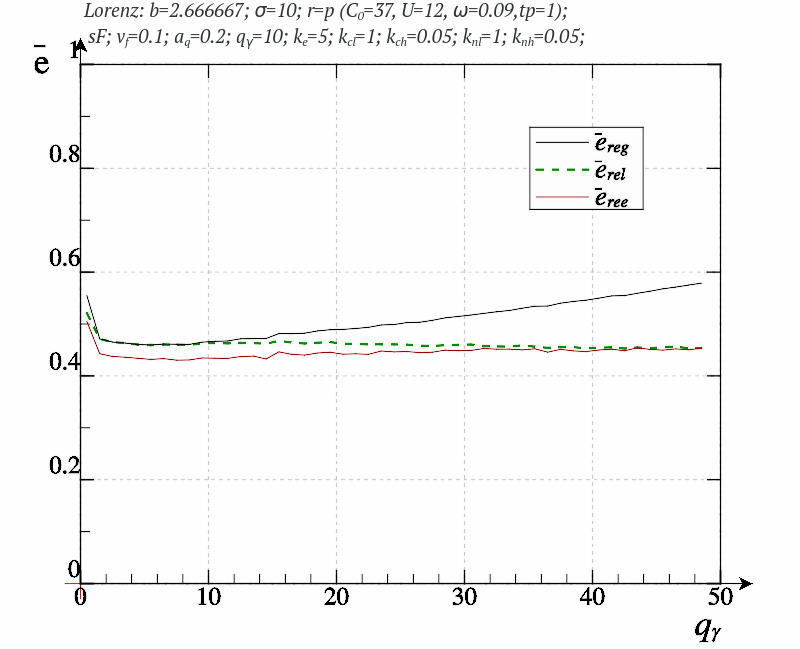
\includegraphics[width=0.49\textwidth]{p/cha/lor/Fq3zlovnAAF/lor_Fq3zlovnAAF_qx2-p_qg_e_sign.png}
    \hfill
    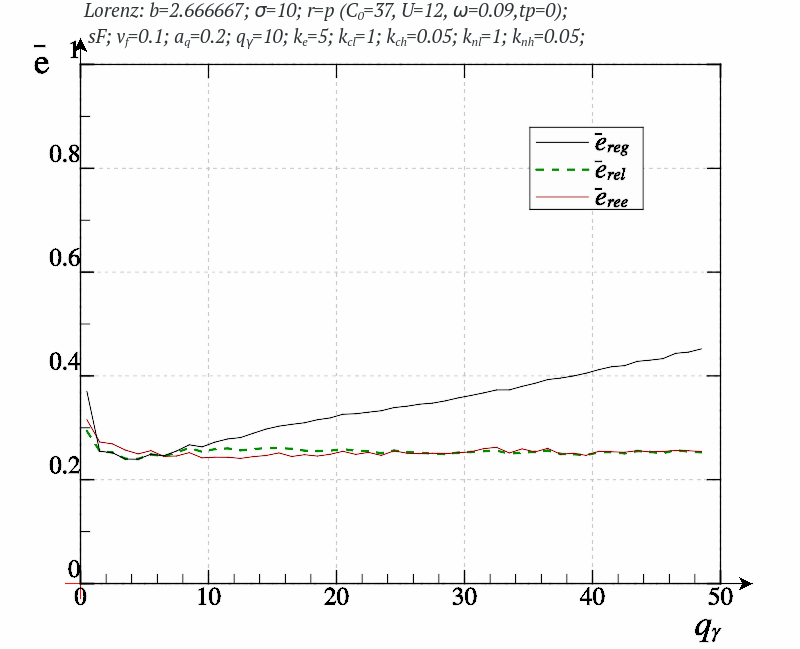
\includegraphics[width=0.49\textwidth]{p/cha/lor/Fq3zlovnAAF/lor_Fq3zlovnAAF_qx2-p_qg_e_sin.png}
  }
\caption{Залежності $ \overline{e}_{r *} (q_\gamma) $ при ідентифікації системи Лоренца методом Fq3zlovnAAF.$q_{x^2} $ при~(\ref{atu:eq:lor_po_t_sign}) і (\ref{atu:eq:lor_po_t_sin})}
\label{atu:f:lor_qg_Fq3zlovnAAF.q_x2}
\end{figure}


Ще один важливий параметр, що впливає на динамічний властивості
системи ідентифікації ---
$ v_f $, який визначає швидкість зсуву агента до обраному значенням
при постійній силі. При нульовому значенні цього коефіцієнта
агенти нерухомі, і можна визначити величину
$ \overline{e}_{be} $, а якщо ще гранично зменшити
$ q_\gamma $ ---
$ \overline{e}_{bb} $.



На рис.~\ref{atu:f:lor_vf_ql3ruonAAF.q_x2} представлені залежності усереднених
помилок ідентифікації системи Лоренца від
$ v_f $ при використанні методу
ql3ruonAAF.$q_{x^2}$.
За винятком початкового ділянки, де рухливість агентів
мінімальна, залежність від
$ v_f $ досить слабка. У міру збільшення
$ v_f $ трохи поліпшуються динамічні властивості, але зростаюча
швидкість переміщення агентів дещо нівелює цей ефект. При
плавній зміні параметра, негативний ефект від надлишкової
рухливості агентів переважає.

\begin{figure}[ht!]
  \centerline{
    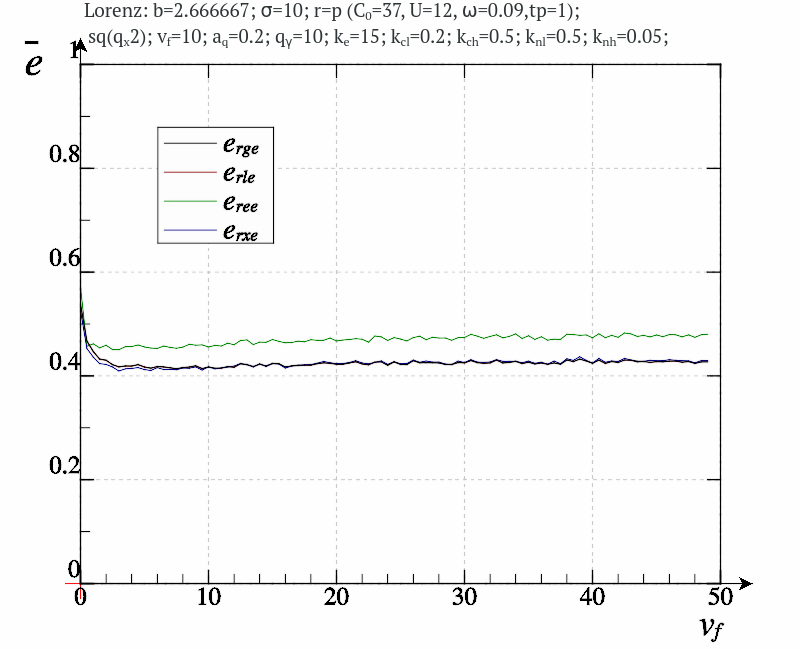
\includegraphics[width=0.49\textwidth]{p/cha/lor/ql3ruonAAF/lor_ql3ruonAAF_qx2-p_v_f_e_sign.png}
    \hfill
    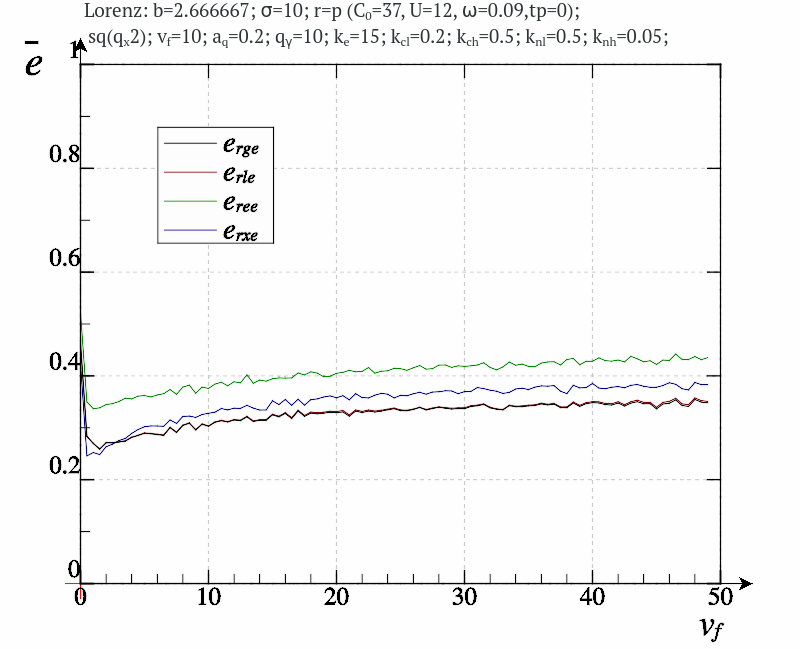
\includegraphics[width=0.49\textwidth]{p/cha/lor/ql3ruonAAF/lor_ql3ruonAAF_qx2-p_v_f_e_sin.png}
  }
\caption{Залежності $ \overline{e}_{r *} (v_f) $ при ідентифікації системи Лоренца методом ql3ruonAAF.$q_{x^2} $ при~(\ref{atu:eq:lor_po_t_sign}) і (\ref{atu:eq:lor_po_t_sin})}
  \label{atu:f:lor_vf_ql3ruonAAF.q_x2}
\end{figure}

Абсолютно аналогічна картина (рис.~\ref{atu:f:lor_vf_ql3ruonAAF.q_y2})
спостерігається при використанні критерію
$q_{y^2}$.
При цьому слід зазначити, що при надмірній рухливості менше
значення похибки демонструють підхід, засновані на глобальному
оцінюванні
$ p_\mathrm{id} $.


\begin{figure}[ht!]
  \centerline{
    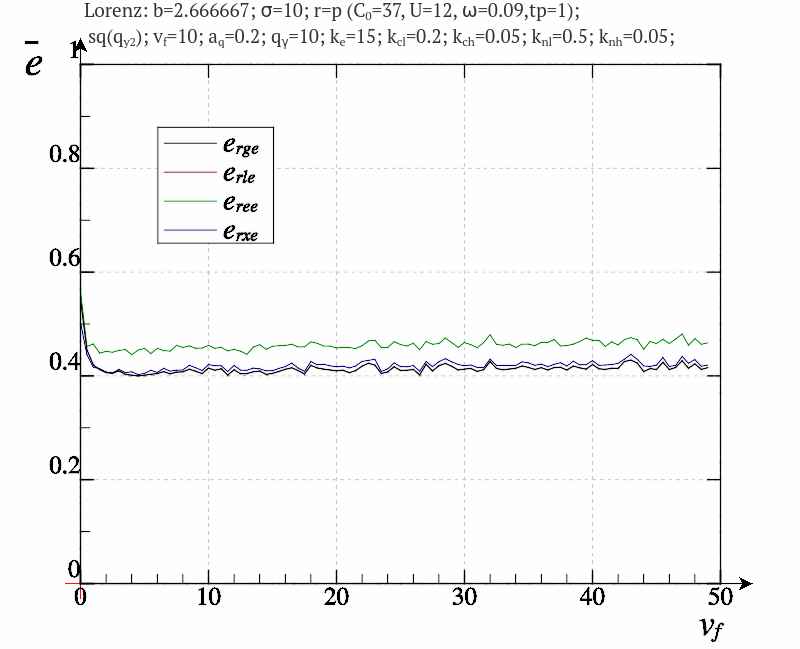
\includegraphics[width=0.49\textwidth]{p/cha/lor/ql3ruonAAF/lor_ql3ruonAAF_qy2-p_v_f_e_sign.png}
    \hfill
    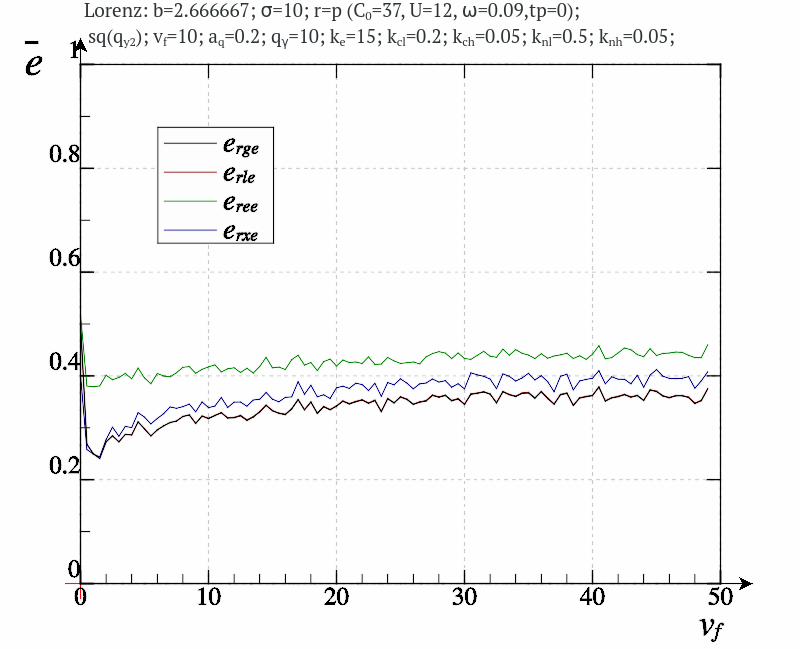
\includegraphics[width=0.49\textwidth]{p/cha/lor/ql3ruonAAF/lor_ql3ruonAAF_qy2-p_v_f_e_sin.png}
  }
\caption{Залежності $ \overline{e}_{r *} (v_f) $ при ідентифікації системи Лоренца методом ql3ruonAAF.$q_{y^2} $ при~(\ref{atu:eq:lor_po_t_sign}) і (\ref{atu:eq:lor_po_t_sin})}
\label{atu:f:lor_vf_ql3ruonAAF.q_y2}
\end{figure}

Дещо інша картина спостерігається при використанні методу
Fq3zlovnAAF.$q_{x^2}$
(рис.~\ref{atu:f:lor_vf_Fq3zlovnAAF.q_x2}).
У досить широкому діапазоні залежність досить слабка, а
велика швидкість призводить до порушення процесу пошуку, що
спостерігається в правій частині обох графіків.

\begin{figure}[ht!]
  \centerline{
    \includegraphics[width=0.49\textwidth]{p/cha/lor/Fq3zlovnAAF/lor_Fq3zlovnAAF_qx2-p_v_f_e_sign.png}
    \hfill
    \includegraphics[width=0.49\textwidth]{p/cha/lor/Fq3zlovnAAF/lor_Fq3zlovnAAF_qx2-p_v_f_e_sin.png}
  }
\caption{Залежності $ \overline{e}_{r *} (v_f) $ при ідентифікації системи Лоренца методом Fq3zlovnAAF.$q_{x^2} $ при~(\ref{atu:eq:lor_po_t_sign}) і (\ref{atu:eq:lor_po_t_sin})}
\label{atu:f:lor_vf_Fq3zlovnAAF.q_x2}
\end{figure}

Останній з параметрів, який заслуговують пильну увагу ---
$ k_e $, задає баланс сил при зміщенні агентів. Слід
зазначити, що в розглянутих прикладах його вплив різний ---
в ql3ruonAAF.$q_{x^2}$ та ql3ruonAAF.$q_{y^2}$
залежність $f_e(p_c-p_e)$ с насиченням,
а у Fq3zlovnAAF.$q_{x^2}$ ця залежність линійна.

На рис.~\ref{atu:f:lor_ke_ql3ruonAAF.q_x2} представлені залежності усереднених
помилок ідентифікації системи Лоренца від
$k_e$ при використанні методу ql3ruonAAF.$q_{x^2} $. Малі значення цього коефіцієнта призводять до тех же
наслідків, що і малі значення $ v_f $ --- агенти стають практично нерухомими.

\begin{figure}[ht!]
  \centerline{
    \includegraphics[width=0.49\textwidth]{p/cha/lor/ql3ruonAAF/lor_ql3ruonAAF_qx2-p_k_e_e_sign.png}
    \hfill
    \includegraphics[width=0.49\textwidth]{p/cha/lor/ql3ruonAAF/lor_ql3ruonAAF_qx2-p_k_e_e_sin.png}
  }
\caption{Залежності $ \overline{e}_{r *} (k_e) $ при ідентифікації системи Лоренца методом ql3ruonAAF.$q_{x^2} $ при~(\ref{atu:eq:lor_po_t_sign}) і (\ref{atu:eq:lor_po_t_sin})}
\label{atu:f:lor_ke_ql3ruonAAF.q_x2}
\end{figure}

Порушення процесу пошуку при використанні критерію
$ q_{y^2} $~рис.~\ref{atu:f:lor_ke_ql3ruonAAF.q_y2} відбувається помітно раніше,
ніж при використанні
$ q_{y^2} $. Це ще раз підтверджує менший діапазон придатності
$ q_{y^2} $.

\begin{figure}[ht!]
  \centerline{
    \includegraphics[width=0.49\textwidth]{p/cha/lor/ql3ruonAAF/lor_ql3ruonAAF_qy2-p_k_e_e_sign.png}
    \hfill
    \includegraphics[width=0.49\textwidth]{p/cha/lor/ql3ruonAAF/lor_ql3ruonAAF_qy2-p_k_e_e_sin.png}
  }
\caption{Залежності $ \overline{e}_{r *} (k_e) $ при ідентифікації системи Лоренца методом ql3ruonAAF.$q_{y^2} $ при~(\ref{atu:eq:lor_po_t_sign}) і (\ref{atu:eq:lor_po_t_sin})}
\label{atu:f:lor_ke_ql3ruonAAF.q_y2}
\end{figure}

На рис.~\ref{atu:f:lor_ke_Fq3zlovnAAF.q_x2} представлені аналогічні залежності
для методу Fq3zlovnAAF.$q_{x^2} $. При загальній подібній структурі залежності
спостерігається порушення пошуку і при вдвічі більшому значенні
даного коефіцієнта.

\begin{figure}[ht!]
  \centerline{
    \includegraphics[width=0.49\textwidth]{p/cha/lor/Fq3zlovnAAF/lor_Fq3zlovnAAF_qx2-p_ke_e_sign.png}
    \hfill
    \includegraphics[width=0.49\textwidth]{p/cha/lor/Fq3zlovnAAF/lor_Fq3zlovnAAF_qx2-p_ke_e_sin.png}
  }
\caption{Залежності $ \overline{e}_{r *} (k_e) $ при ідентифікації системи Лоренца методом Fq3zlovnAAF.$q_{x^2} $ при~(\ref{atu:eq:lor_po_t_sign}) і (\ref{atu:eq:lor_po_t_sin})}
\label{atu:f:lor_ke_Fq3zlovnAAF.q_x2}
\end{figure}


% }}}2


% ----------------------------------------- F_type -------------------------------

\subsection{Вплив виду функції якості на процес ідентифікації}%{{{2

Розглянемо вплив типу функції якості на властивості системи
ідентифікації. Для цього розглянемо сімейство залежностей
$ \overline{e} (q_\gamma) $ для різних видів
$ F (q) $ (\ref{atu:eq:F_gauss}) --- (\ref{atu:eq:F_log}) . Для даного дослідження обрано
метод Fq3zlovnAAF.$q_{x^2} $, як безпосередньо використовує функцію якості при
апроксимації $ p_e $. З усіх видів залежностей вибрана саме ці, так як
$ q_\gamma $ безпосередньо входить у визначення функції якості.


На рис.~\ref{atu:f:lor_ftype_rge} представлені
$ \overline{e}_{rge} (q_\gamma) $ при використанні методу
Fq3zlovnAAF.$q_{x^2}$.
Слід зазначити, що в цьому випадку функція якості
використовується два рази: перший раз в кожному агенті при
визначенні
$ p_e $, другий --- при визначенні глобального
$ p_{ge} $. Саме цей вплив пояснює плавний простий похибки
ідентифікації при зростанні
$ q_\gamma $, і отже, зменшення чутливості в правій частині графіків. У
лівій частині графіків спостерігаються істотні відмінності
при використанні різних видів функцій якості. Застосування
параболічної, трикутної і логарифмічною залежностей
призводить до різкого зростання похибки при збільшенні
чутливості. Гіперболічна і гауссова залежності залишаються
застосовні і при підвищеній чутливості функції якості.

\begin{figure}[ht!]
  \centerline{
    \includegraphics[width=0.49\textwidth]{p/cha/lor/Fq3zlovnAAF/f_type/lor_Fq3zlovnAAF_qx2_Ft-p_qg_e_all_sign_rge.png}
    \hfill
    \includegraphics[width=0.49\textwidth]{p/cha/lor/Fq3zlovnAAF/f_type/lor_Fq3zlovnAAF_qx2_Ft-p_qg_e_all_sin_rge.png}
  }
\caption{Сімейства залежностей $ \overline{e}_{rge} (q_\gamma) $ для різних видів функцій якості при ідентифікації системи Лоренца методом Fq3zlovnAAF.$q_{x^2} $ при~(\ref{atu:eq:lor_po_t_sign}) і (\ref{atu:eq:lor_po_t_sin})}
\label{atu:f:lor_ftype_rge}
\end{figure}

На рис.~\ref{atu:f:lor_ftype_ree} представлені
$ \overline{e}_{rge} (q_\gamma) $ при використанні методу Fq3zlovnAAF.$q_{x^2} $.
Результати в цілому схожі з попередніми, список
видів функцій якості, що забезпечують більш широкий діапазон
застосовності не змінився. Проте, з огляду на те, що в даному
випадку використовується тільки локальна оцінка, зростання
$ q_\gamma $ в розумних межах не призводить до збільшення похибки
ідентифікації.

\begin{figure}[ht!]
  \centerline{
    \includegraphics[width=0.49\textwidth]{p/cha/lor/Fq3zlovnAAF/f_type/lor_Fq3zlovnAAF_qx2_Ft-p_qg_e_all_sign_ree.png}
    \hfill
    \includegraphics[width=0.49\textwidth]{p/cha/lor/Fq3zlovnAAF/f_type/lor_Fq3zlovnAAF_qx2_Ft-p_qg_e_all_sin_ree.png}
  }
  \caption{Сімейства залежностей $ \overline{e}_{ree} (q_\gamma) $ для різних видів функцій якості при ідентифікації системи Лоренца методом Fq3zlovnAAF.$q_{x^2} $ при~(\ref{atu:eq:lor_po_t_sign}) і (\ref{atu:eq:lor_po_t_sin})}
  \label{atu:f:lor_ftype_ree}
\end{figure}

Таким чином, результати моделювання при використанні функцій
якості видів (\ref{atu:eq:F_gauss})--(\ref{atu:eq:F_log}) показують, що при
порівняно однакових результатах в широкому діапазоні
$ q_\gamma $, кращі результати в цілому демонструють функції
(\ref{atu:eq:F_hyper}) і (\ref{atu:eq:F_gauss}), за рахунок кращої роботи в області
високої чутливості. А так як в цілому застосування гіперболічної
залежності призводить нехай до несуттєво, але більшої похибки
ідентифікації в цілому, то в подальшому будемо застосовувати
функцію якості у вигляді~(\ref{atu:eq:F_gauss}).

% }}}2


% ----------------------------------------- N -------------------------------

\subsection{Вплив кількості пошукових агентів на процес ідентифікації} % {{{2

Розглянемо вплив кількості пошукових агентів на якість
ідентифікації на прикладі сімейства методів
Fq3zlovnAAF.$q_{x^2}$.
Структура зв'язків пошукових агентів визначає їх мінімальну кількість
$ N = 3 $, не рахуючи двох нерухомих моделей на границі. Розглянемо
випадки $ N = 3,5,7,9 $.

В першу чергу відзначимо, що з усіх параметрів даної системи
ідентифікації найтісніший і безпосередній зв'язок з кількістю
агентів має параметр $ q_\gamma $.
Це повинно пояснюється тим, що чим більше агентів на
$ \mathcal{P} $, тим менше між ними відстань в просторі параметрів, і
отже, значення критеріїв ідентифікації розрізняються менше,
що, в свою чергу, вимагає більшої чутливості.

Розглянемо отримані залежності. На рис.~\ref{atu:f:lor_N_rge} представлені
$ \overline{e}_{rge} (q_\gamma) $ для різних
$ N $. Тут отримані, на перший погляд, парадоксальні результати. В
обох випадках, при відносно великих значеннях
$ q_\gamma $, система ідентифікації з трьома моделями показує кращі
результати. Насправді, ніякого парадоксу в отриманих даних
немає. При визначенні
$ p_{ge} $, а отже, а
$ \overline{e}_{rge} $ враховується внесок всіх моделей, в тому числі і
розташованих далеко від
$ p_o $. При великих значеннях
$ q_\gamma $, і отже, при низькій чутливості, внесок ``далеких''
моделей зростає, і, чим більше моделей, тим більше цей
внесок. При нормальній чутливості (ліва частина графіків), цей
ефект практично зникає. Проте, для даних умов, використання
кількості моделей
$ N> 5 $ недоцільно.



\begin{figure}[ht!]
  \centerline{
    \includegraphics[width=0.49\textwidth]{p/cha/lor/Fq3zlovnAAF/N/lor_Fq3zlovnAAF_qx2_p_qg_e_rge_sign.png}
    \hfill
    \includegraphics[width=0.49\textwidth]{p/cha/lor/Fq3zlovnAAF/N/lor_Fq3zlovnAAF_qx2_p_qg_e_rge_sin.png}
  }
\caption{Сімейства залежностей $ \overline{e}_{rge} (q_\gamma) $ для різних значень $ N $ при ідентифікації системи Лоренца методом Fq3zlovnAAF.$ q_{x^2} $ при~(\ref{atu:eq:lor_po_t_sign}) і (\ref{atu:eq:lor_po_t_sin})}
\label{atu:f:lor_N_rge}
\end{figure}


Застосування локальних методів оцінювання
$ p_\mathrm{id} $, з обмеженою кількістю використовуваних моделей,
не повинно бути піддано цьому явищу. Для перевірки цієї тези
розглянемо залежності
$ \overline{e}_{ree} (q_\gamma) $ представлені на рис.~\ref{atu:f:lor_N_rge} для того
ж набору $ N $.

\begin{figure}[ht!]
  \centerline{
    \includegraphics[width=0.49\textwidth]{p/cha/lor/Fq3zlovnAAF/N/lor_Fq3zlovnAAF_qx2_p_qg_e_ree_sign.png}
    \hfill
    \includegraphics[width=0.49\textwidth]{p/cha/lor/Fq3zlovnAAF/N/lor_Fq3zlovnAAF_qx2_p_qg_e_ree_sin.png}
  }
\caption{Сімейства залежностей $ \overline{e}_{ree} (q_\gamma) $ для різних значень
$ N $ при ідентифікації системи Лоренца методом Fq3zlovnAAF.$q_{x^2} $ при~(\ref{atu:eq:lor_po_t_sign}) і (\ref{atu:eq:lor_po_t_sin})}
\label{atu:f:lor_N_ree}
\end{figure}

В цьому випадку при великих значеннях
$ q_\gamma $ всі розглянуті похибки ідентифікації практично
збігаються, і проявляють досить слабку залежність. У лівій
частині графіків, система з
$ N = 3 $ помітно програє системі з
$ N = 5 $, а інші не перевершують останню.

% }}}2


% ----------------------------------------- multi param -------------------------------

\subsection{Залежності значень критеріїв ідентифікації при зміні двох параметрів системи Лоренца} % {{{2

Для оцінки можливості одночасної ідентифікації декількох параметрів
розглянуто графіки залежностей критеріїв за умови зміни двох параметрів
попарно: ($r$, $\sigma$) і ($r$, $b$).
%
При цьому скористається структурою системи~(\ref{atu:eq:lor}) і введемо
ще один додатковий критерій:$ q_{(x-y)^2} $.

На рис.~\ref{atu:f:lor_qx2_r_b} приведена залежність
$ q_{x^2} (r, b) $. Аналіз виду цієї поверхні дозволяє зробити
висновок, що одного цього критерію недостатньо для одночасної
ідентифікації параметрів
$ r $ і
$ b $. Явно виражений ``яр'' на графіку відповідає переходу з режиму
загасання в хаотичний, отже, не має принципового значення.

\begin{figure}[ht!]
  \centerline{  \includegraphics[width=0.60\textwidth]{p/cha/lor/q2d/lor_qx2_r_b.png}  }
  \caption{Залежність $ q_{x^2} (r, b) $ для системи Лоренца}
  \label{atu:f:lor_qx2_r_b}
\end{figure}


На рис.~\ref{atu:f:lor_qy2_r_b} приведена залежність
$ q_{y^2} (r, b) $. Вид цієї поверхні практично не відрізняється від
попередньої. При цьому абсолютно не спостерігається ніяких
очевидних причин виявленого в попередніх дослідженнях більш
вузькому діапазону застосовності даного критерію.

\begin{figure}[ht!]
  \centerline{  \includegraphics[width=0.60\textwidth]{p/cha/lor/q2d/lor_qy2_r_b.png}  }
  \caption{Залежність $ q_{y^2} (r, b) $ для системи Лоренца}
  \label{atu:f:lor_qy2_r_b}
\end{figure}

На рис.~\ref{atu:f:lor_qz2_r_b} приведена залежність
$q_{z^2}(r,b)$.
Вид цієї залежності істотно відрізняється від двох попередніх.
Близька до квадратичної залежність від параметра $r$ не представляє особливих
проблем. Корисним є той факт, що для даного критерію залежність від параметра $b$
досить мала. Отже, при двопараметричной ідентифікації даний критерій має
сенс використовувати для (оціночної) ідентифікації параметра $r$, і
сукупність даного критерію разом з, наприклад, $q_{x^2}$ дозволить
ідентифікувати обидва параметри без використання надмірної кількості моделей.

\begin{figure}[ht!]
  \centerline{  \includegraphics[width=0.60\textwidth]{p/cha/lor/q2d/lor_qz2_r_b.png}  }
  \caption{Залежність $ q_{z^2} (r, b) $ для системи Лоренца}
  \label{atu:f:lor_qz2_r_b}
\end{figure}

На рис.~\ref{atu:f:lor_qxmy2_r_b} приведена залежність
$q_{(x-y)^2}(r,b)$.
Очевидно, що для ідентифікації даний критерій практично
непридатний, проте, він відмінний від нуля тільки там, де система
не знаходиться в режимі загасання, що може бути корисно для
швидкого визначення режиму роботи.

\begin{figure}[ht!]
  \centerline{  \includegraphics[width=0.60\textwidth]{p/cha/lor/q2d/lor_qxmy2_r_b.png}  }
  \caption{Залежність $ q_{(x-y)^2} (r, b) $ для системи Лоренца}
  \label{atu:f:lor_qxmy2_r_b}
\end{figure}


На рис.~\ref{atu:f:lor_qx2_r_sigma} приведена залежність
$q_{x^2}(r,\sigma)$.
Поведінка цього критерію на парі параметрів
$ (r, \sigma) $ істотно відрізняється від його ж поведінки на парі
$ (r, b) $. За винятком вузького ``яру'', залежність від параметра
$ \sigma $ мала, що дає підстави для незалежної ідентифікації
параметра~$r$.

\begin{figure}[ht!]
  \centerline{  \includegraphics[width=0.60\textwidth]{p/cha/lor/q2d/lor_qx2_r_sigma.png}  }
  \caption{Залежність $ q_{x^2} (r, \sigma) $ для системи Лоренца}
  \label{atu:f:lor_qx2_r_sigma}
\end{figure}


На рис.~\ref{atu:f:lor_qy2_r_sigma} приведена залежність
$q_{y^2}(r,\sigma)$.
Ця залежність в цілому схожа на попередню, проте, на місці ``яру'' спостерігається ``хребет''.

\begin{figure}[ht!]
  \centerline{  \includegraphics[width=0.60\textwidth]{p/cha/lor/q2d/lor_qy2_r_sigma.png}  }
  \caption{Залежність $ q_{y^2} (r, \sigma) $ для системи Лоренца}
  \label{atu:f:lor_qy2_r_sigma}
\end{figure}

На рис.~\ref{atu:f:lor_qz2_r_sigma} приведена залежність
$ q_{z^2} (r, \sigma) $. На відміну від застосування даного критерію
на парі
$ (r, b) $, не спостерігається принципової різниці між даним
критерієм, і критерієм
$ q_{x^2} $. Відсутність суттєвої різниці не дає достатніх підстав
для одночасної ідентифікації пари параметрів
$ (r, \sigma) $ із застосуванням тільки цих двох критеріїв.

\begin{figure}[ht!]
  \centerline{  \includegraphics[width=0.60\textwidth]{p/cha/lor/q2d/lor_qz2_r_sigma.png}  }
  \caption{Зависимость $q_{z^2}(r,\sigma)$ для системы Лоренца}
  \label{atu:f:lor_qz2_r_sigma}
\end{figure}

На рис.~\ref{atu:f:lor_qxmy2_r_sigma} приведена залежність
$ q_{(x-y)^2} (r, \sigma) $. Ця залежність принципово не відрізняється
від представленої на рис.~(\ref{atu:f:lor_qxmy2_r_b}), за винятком того, що
присутен ``хребет''.

\begin{figure}[ht!]
  \centerline{  \includegraphics[width=0.60\textwidth]{p/cha/lor/q2d/lor_qxmy2_r_sigma.png}  }
  \caption{Залежність $ q_{(x-y)^2} (r, \sigma) $ для системи Лоренца}
  \label{atu:f:lor_qxmy2_r_sigma}
\end{figure}

% }}}2


\subsection{Выводы}  % {{{2

Результати моделювання як власне динаміки системи Лоренца,
так і процесів ідентифікації параметра ``$r$ '' дозволяють в
цілому зробити наступні висновки:

\begin{itemize}

  \item
    Для синтезу працездатною системи ідентифікації параметра
    ``$r$ '' системи Лоренца можуть застосовуватися практично все
    розглянуті критерії. При цьому, більший діапазон застосовності
    --- у критерію~$ q_{x^2} $.

  \item
    Система мультиагентной ідентифікації може бути реалізована
    як з агентами, які здійснюють пошук як з використанням
    критерію, так і з використанням функції якості. При цьому,
    похибка ідентифікації визначається в основному не конкретним
    методом, а динамічними властивостями самого ідентифікованого
    об'єкта і використовуваним часом усереднення критерію.

  \item
    Для розглянутого типу об'єктів більшість параметрів системи
    ідентифікації дозволяють зміни в досить широкому діапазоні
    без втрати працездатності, що спрощує застосування системи
    ідентифікації у випадках, коли немає можливості проводити
    широкий набір попередніх вимірювань. Винятком є параметр
    $a_q$, при цьому його допустимий діапазон визначається динамічним
    властивостями об'єкта.

  \item
    Застосування функції якості у вигляді~(\ref{atu:eq:F_gauss}) дозволяє в
    цілому отримати кращі результати ідентифікації.

  \item
    Існує певна кількість агентів, перевищення якого не збільшує
    якість ідентифікації, а в деяких випадках, наприклад, при
    використанні глобальних методів оцінювання
    $p_\mathrm{id} $ і низької чутливості, призводить до погіршення
    властивостей системи ідентифікації.

  \item
    Можлива одночасна ідентифікація параметрів
    $ r $ і
    $ b $, за умови спільного застосування критеріїв
    $ q_{x^2} $ і
    $ q_{z^2} $.

\end{itemize}

% }}}2


% }}}1




% habr: 
% 1. Конвекция в тороидальной трубе (Ланда П.С. Нелинейные колебания и волны. — М: Либроком, 2010, с. 454-455)
% 2. Одномодовый лазер (Покровский Л.А. Решение системы уравнений Лоренца в
%  асимптотическом пределе большого числа Релея. I. Система Лоренца в простейшей
%  квантовой модели лазера и приложение к ней метода усреднения // Теоретическая
%  и математическая физика, 1985, т. 62, №2, с. 272-290);
% 3. Осциллятор с инерционным возбуждением (Неймарк Ю.И., Ланда П.С.
% Стохастические и хаотические колебания. — М: Либроком, 2009, с. 288-295).

% vim: fdm=marker foldlevel=1 foldignore="%#" fdc=4 ft=tex
